This section covers basic performance tests, i.e. how specific algorithms scale
with grid resolution or with polynomial degree, on a \emph{single compute node}.

% --------------------------------------------------------------------------------
\section{Solver Performance - Poisson problems}
\label{sec:SolverPerformancePoisson}
% --------------------------------------------------------------------------------
Three different groups of solvers are compared:
\begin{itemize}
\item
Direct Solvers: directs sparse methods, such as PARDISO\footnote{
\url{http://www.pardiso-project.org/}}
and MUMPS\footnote{
\url{http://mumps.enseeiht.fr/}}
are compared.
Their performance also serves as a comparative baseline.

\item
Iterative Algorithms without preconditioning, resp. low-impact, generic preconditioning:
This includes solver libraries such as \code{monkey} (BoSSS-specific, supports GPU)
as well as
HYPRE\footnote{
\url{https://computation.llnl.gov/projects/hypre-scalable-linear-solvers-multigrid-methods}}
(native library, used via wrappers).

\item
Iterative Algorithms with \ac{dg}-specific preconditioners, such as aggregation multigrid
and multi-level additive Schwarz
\end{itemize}


\subsection{Constant Diffusion Coefficient test problem}
\label{sec:ConstantDiffusionCoefficient}
The problem
\begin{equation}
\left\{ \begin{array} {rclll}
- \Delta T   & = & g_{\domain}                      
& \text{in}\ \Omega = (0,10) \times (-1,1) \times (-1,1)  &  \\
% ----
T   & = & g_D = 0                             
& \text{on}\ \Gamma_D = \{ (x,y,z) \in \real^3; \ x = 0 \}
& \text{Dirichlet-boundary} \\
% ----
\nabla T \cdot \vec{n}_{\partial \domain} & = & g_N 
& \text{on}\ \Gamma_N = \partial \Omega \setminus \Gamma_D
& \text{Neumann-boundary}
\end{array} \right.
\label{eq:ContantCoeffPoissonBenchmark}
\end{equation}
is investigated on a non-uniform, Cartesian grid
(equidistant in $z$, sinus-spacing in $x$ and $y$ direction).
The large $\Gamma_N$ makes the problem harder for non-preconditioned
iterative methods. See Figure \ref{fig:ConstantCoeffRuntimes} for results.

\graphicspath{{./apdx-NodeSolverPerformance/PoissonConstCoeff/plots/}}

Subsequent the performance of some code parts are investigated for the block Jacobian and the Schwarz multigrid preconditioned conjugate gradient method (PCG):
\begin{itemize}
	\item MatrixAssembly: assemble Block matrix
	\item Aggregation basis init: create multigrid sequence, contains information about the transformation at the multigrid levels
	\item Solver Init: hand over/assemble relevant data for the chosen solver, e.g. operator matrix etc.
	\item Solver Run: solves the equation system: operator matrix, vector of dg coordinates and given RHS 
\end{itemize}
Both variants are using pre and post smoothing solvers (5 runs at each multigrid level).



\begin{figure}[!h]
	\begin{center}
		% GNUPLOT: LaTeX picture with Postscript
\begingroup
  \makeatletter
  \providecommand\color[2][]{%
    \GenericError{(gnuplot) \space\space\space\@spaces}{%
      Package color not loaded in conjunction with
      terminal option `colourtext'%
    }{See the gnuplot documentation for explanation.%
    }{Either use 'blacktext' in gnuplot or load the package
      color.sty in LaTeX.}%
    \renewcommand\color[2][]{}%
  }%
  \providecommand\includegraphics[2][]{%
    \GenericError{(gnuplot) \space\space\space\@spaces}{%
      Package graphicx or graphics not loaded%
    }{See the gnuplot documentation for explanation.%
    }{The gnuplot epslatex terminal needs graphicx.sty or graphics.sty.}%
    \renewcommand\includegraphics[2][]{}%
  }%
  \providecommand\rotatebox[2]{#2}%
  \@ifundefined{ifGPcolor}{%
    \newif\ifGPcolor
    \GPcolortrue
  }{}%
  \@ifundefined{ifGPblacktext}{%
    \newif\ifGPblacktext
    \GPblacktexttrue
  }{}%
  % define a \g@addto@macro without @ in the name:
  \let\gplgaddtomacro\g@addto@macro
  % define empty templates for all commands taking text:
  \gdef\gplbacktext{}%
  \gdef\gplfronttext{}%
  \makeatother
  \ifGPblacktext
    % no textcolor at all
    \def\colorrgb#1{}%
    \def\colorgray#1{}%
  \else
    % gray or color?
    \ifGPcolor
      \def\colorrgb#1{\color[rgb]{#1}}%
      \def\colorgray#1{\color[gray]{#1}}%
      \expandafter\def\csname LTw\endcsname{\color{white}}%
      \expandafter\def\csname LTb\endcsname{\color{black}}%
      \expandafter\def\csname LTa\endcsname{\color{black}}%
      \expandafter\def\csname LT0\endcsname{\color[rgb]{1,0,0}}%
      \expandafter\def\csname LT1\endcsname{\color[rgb]{0,1,0}}%
      \expandafter\def\csname LT2\endcsname{\color[rgb]{0,0,1}}%
      \expandafter\def\csname LT3\endcsname{\color[rgb]{1,0,1}}%
      \expandafter\def\csname LT4\endcsname{\color[rgb]{0,1,1}}%
      \expandafter\def\csname LT5\endcsname{\color[rgb]{1,1,0}}%
      \expandafter\def\csname LT6\endcsname{\color[rgb]{0,0,0}}%
      \expandafter\def\csname LT7\endcsname{\color[rgb]{1,0.3,0}}%
      \expandafter\def\csname LT8\endcsname{\color[rgb]{0.5,0.5,0.5}}%
    \else
      % gray
      \def\colorrgb#1{\color{black}}%
      \def\colorgray#1{\color[gray]{#1}}%
      \expandafter\def\csname LTw\endcsname{\color{white}}%
      \expandafter\def\csname LTb\endcsname{\color{black}}%
      \expandafter\def\csname LTa\endcsname{\color{black}}%
      \expandafter\def\csname LT0\endcsname{\color{black}}%
      \expandafter\def\csname LT1\endcsname{\color{black}}%
      \expandafter\def\csname LT2\endcsname{\color{black}}%
      \expandafter\def\csname LT3\endcsname{\color{black}}%
      \expandafter\def\csname LT4\endcsname{\color{black}}%
      \expandafter\def\csname LT5\endcsname{\color{black}}%
      \expandafter\def\csname LT6\endcsname{\color{black}}%
      \expandafter\def\csname LT7\endcsname{\color{black}}%
      \expandafter\def\csname LT8\endcsname{\color{black}}%
    \fi
  \fi
    \setlength{\unitlength}{0.0500bp}%
    \ifx\gptboxheight\undefined%
      \newlength{\gptboxheight}%
      \newlength{\gptboxwidth}%
      \newsavebox{\gptboxtext}%
    \fi%
    \setlength{\fboxrule}{0.5pt}%
    \setlength{\fboxsep}{1pt}%
\begin{picture}(7920.00,6800.00)%
    \gplgaddtomacro\gplbacktext{%
      \csname LTb\endcsname%
      \put(997,4825){\makebox(0,0)[r]{\strut{}$10^{-2}$}}%
      \csname LTb\endcsname%
      \put(997,5150){\makebox(0,0)[r]{\strut{}$10^{-1}$}}%
      \csname LTb\endcsname%
      \put(997,5475){\makebox(0,0)[r]{\strut{}$10^{0}$}}%
      \csname LTb\endcsname%
      \put(997,5800){\makebox(0,0)[r]{\strut{}$10^{1}$}}%
      \csname LTb\endcsname%
      \put(997,6126){\makebox(0,0)[r]{\strut{}$10^{2}$}}%
      \csname LTb\endcsname%
      \put(997,6451){\makebox(0,0)[r]{\strut{}$10^{3}$}}%
      \csname LTb\endcsname%
      \put(997,6776){\makebox(0,0)[r]{\strut{}$10^{4}$}}%
      \csname LTb\endcsname%
      \put(1099,4646){\makebox(0,0){\strut{} }}%
      \csname LTb\endcsname%
      \put(2137,4646){\makebox(0,0){\strut{} }}%
      \csname LTb\endcsname%
      \put(3176,4646){\makebox(0,0){\strut{} }}%
      \csname LTb\endcsname%
      \put(4214,4646){\makebox(0,0){\strut{} }}%
      \csname LTb\endcsname%
      \put(5252,4646){\makebox(0,0){\strut{} }}%
      \csname LTb\endcsname%
      \put(6291,4646){\makebox(0,0){\strut{} }}%
      \csname LTb\endcsname%
      \put(7329,4646){\makebox(0,0){\strut{} }}%
      \csname LTb\endcsname%
      \put(7431,4825){\makebox(0,0)[l]{\strut{} }}%
      \csname LTb\endcsname%
      \put(7431,5150){\makebox(0,0)[l]{\strut{} }}%
      \csname LTb\endcsname%
      \put(7431,5475){\makebox(0,0)[l]{\strut{} }}%
      \csname LTb\endcsname%
      \put(7431,5801){\makebox(0,0)[l]{\strut{} }}%
      \csname LTb\endcsname%
      \put(7431,6126){\makebox(0,0)[l]{\strut{} }}%
      \csname LTb\endcsname%
      \put(7431,6451){\makebox(0,0)[l]{\strut{} }}%
      \csname LTb\endcsname%
      \put(7431,6776){\makebox(0,0)[l]{\strut{} }}%
    }%
    \gplgaddtomacro\gplfronttext{%
      \csname LTb\endcsname%
      \put(397,5800){\rotatebox{-270}{\makebox(0,0){\strut{}$k = 2$}}}%
      \csname LTb\endcsname%
      \put(2190,6565){\makebox(0,0)[l]{\strut{}GMRES w. pTG}}%
      \csname LTb\endcsname%
      \put(2190,6286){\makebox(0,0)[l]{\strut{}Kcycle w. add.-Schwarz}}%
      \csname LTb\endcsname%
      \put(2190,6007){\makebox(0,0)[l]{\strut{}Pardiso}}%
      \csname LTb\endcsname%
      \put(2190,5728){\makebox(0,0)[l]{\strut{}linear}}%
    }%
    \gplgaddtomacro\gplbacktext{%
      \csname LTb\endcsname%
      \put(997,2558){\makebox(0,0)[r]{\strut{}$10^{-2}$}}%
      \csname LTb\endcsname%
      \put(997,2883){\makebox(0,0)[r]{\strut{}$10^{-1}$}}%
      \csname LTb\endcsname%
      \put(997,3209){\makebox(0,0)[r]{\strut{}$10^{0}$}}%
      \csname LTb\endcsname%
      \put(997,3534){\makebox(0,0)[r]{\strut{}$10^{1}$}}%
      \csname LTb\endcsname%
      \put(997,3859){\makebox(0,0)[r]{\strut{}$10^{2}$}}%
      \csname LTb\endcsname%
      \put(997,4185){\makebox(0,0)[r]{\strut{}$10^{3}$}}%
      \csname LTb\endcsname%
      \put(997,4510){\makebox(0,0)[r]{\strut{}$10^{4}$}}%
      \csname LTb\endcsname%
      \put(1099,2379){\makebox(0,0){\strut{} }}%
      \csname LTb\endcsname%
      \put(2137,2379){\makebox(0,0){\strut{} }}%
      \csname LTb\endcsname%
      \put(3176,2379){\makebox(0,0){\strut{} }}%
      \csname LTb\endcsname%
      \put(4214,2379){\makebox(0,0){\strut{} }}%
      \csname LTb\endcsname%
      \put(5252,2379){\makebox(0,0){\strut{} }}%
      \csname LTb\endcsname%
      \put(6291,2379){\makebox(0,0){\strut{} }}%
      \csname LTb\endcsname%
      \put(7329,2379){\makebox(0,0){\strut{} }}%
      \csname LTb\endcsname%
      \put(7431,2558){\makebox(0,0)[l]{\strut{} }}%
      \csname LTb\endcsname%
      \put(7431,2883){\makebox(0,0)[l]{\strut{} }}%
      \csname LTb\endcsname%
      \put(7431,3209){\makebox(0,0)[l]{\strut{} }}%
      \csname LTb\endcsname%
      \put(7431,3534){\makebox(0,0)[l]{\strut{} }}%
      \csname LTb\endcsname%
      \put(7431,3859){\makebox(0,0)[l]{\strut{} }}%
      \csname LTb\endcsname%
      \put(7431,4185){\makebox(0,0)[l]{\strut{} }}%
      \csname LTb\endcsname%
      \put(7431,4510){\makebox(0,0)[l]{\strut{} }}%
      \csname LTb\endcsname%
      \put(1099,4689){\makebox(0,0){\strut{} }}%
      \csname LTb\endcsname%
      \put(2137,4689){\makebox(0,0){\strut{} }}%
      \csname LTb\endcsname%
      \put(3176,4689){\makebox(0,0){\strut{} }}%
      \csname LTb\endcsname%
      \put(4214,4689){\makebox(0,0){\strut{} }}%
      \csname LTb\endcsname%
      \put(5252,4689){\makebox(0,0){\strut{} }}%
      \csname LTb\endcsname%
      \put(6291,4689){\makebox(0,0){\strut{} }}%
      \csname LTb\endcsname%
      \put(7329,4689){\makebox(0,0){\strut{} }}%
    }%
    \gplgaddtomacro\gplfronttext{%
      \csname LTb\endcsname%
      \put(397,3534){\rotatebox{-270}{\makebox(0,0){\strut{}$k = 3$}}}%
    }%
    \gplgaddtomacro\gplbacktext{%
      \csname LTb\endcsname%
      \put(997,291){\makebox(0,0)[r]{\strut{}$10^{-2}$}}%
      \csname LTb\endcsname%
      \put(997,616){\makebox(0,0)[r]{\strut{}$10^{-1}$}}%
      \csname LTb\endcsname%
      \put(997,942){\makebox(0,0)[r]{\strut{}$10^{0}$}}%
      \csname LTb\endcsname%
      \put(997,1267){\makebox(0,0)[r]{\strut{}$10^{1}$}}%
      \csname LTb\endcsname%
      \put(997,1593){\makebox(0,0)[r]{\strut{}$10^{2}$}}%
      \csname LTb\endcsname%
      \put(997,1918){\makebox(0,0)[r]{\strut{}$10^{3}$}}%
      \csname LTb\endcsname%
      \put(997,2244){\makebox(0,0)[r]{\strut{}$10^{4}$}}%
      \csname LTb\endcsname%
      \put(1099,41){\makebox(0,0){\strut{}$10^{1}$}}%
      \csname LTb\endcsname%
      \put(2137,41){\makebox(0,0){\strut{}$10^{2}$}}%
      \csname LTb\endcsname%
      \put(3176,41){\makebox(0,0){\strut{}$10^{3}$}}%
      \csname LTb\endcsname%
      \put(4214,41){\makebox(0,0){\strut{}$10^{4}$}}%
      \csname LTb\endcsname%
      \put(5252,41){\makebox(0,0){\strut{}$10^{5}$}}%
      \csname LTb\endcsname%
      \put(6291,41){\makebox(0,0){\strut{}$10^{6}$}}%
      \csname LTb\endcsname%
      \put(7329,41){\makebox(0,0){\strut{}$10^{7}$}}%
      \csname LTb\endcsname%
      \put(7431,291){\makebox(0,0)[l]{\strut{} }}%
      \csname LTb\endcsname%
      \put(7431,617){\makebox(0,0)[l]{\strut{} }}%
      \csname LTb\endcsname%
      \put(7431,942){\makebox(0,0)[l]{\strut{} }}%
      \csname LTb\endcsname%
      \put(7431,1268){\makebox(0,0)[l]{\strut{} }}%
      \csname LTb\endcsname%
      \put(7431,1593){\makebox(0,0)[l]{\strut{} }}%
      \csname LTb\endcsname%
      \put(7431,1919){\makebox(0,0)[l]{\strut{} }}%
      \csname LTb\endcsname%
      \put(7431,2244){\makebox(0,0)[l]{\strut{} }}%
      \csname LTb\endcsname%
      \put(1099,2423){\makebox(0,0){\strut{} }}%
      \csname LTb\endcsname%
      \put(2137,2423){\makebox(0,0){\strut{} }}%
      \csname LTb\endcsname%
      \put(3176,2423){\makebox(0,0){\strut{} }}%
      \csname LTb\endcsname%
      \put(4214,2423){\makebox(0,0){\strut{} }}%
      \csname LTb\endcsname%
      \put(5252,2423){\makebox(0,0){\strut{} }}%
      \csname LTb\endcsname%
      \put(6291,2423){\makebox(0,0){\strut{} }}%
      \csname LTb\endcsname%
      \put(7329,2423){\makebox(0,0){\strut{} }}%
    }%
    \gplgaddtomacro\gplfronttext{%
      \csname LTb\endcsname%
      \put(397,1267){\rotatebox{-270}{\makebox(0,0){\strut{}$k = 5$}}}%
    }%
    \gplbacktext
    \put(0,0){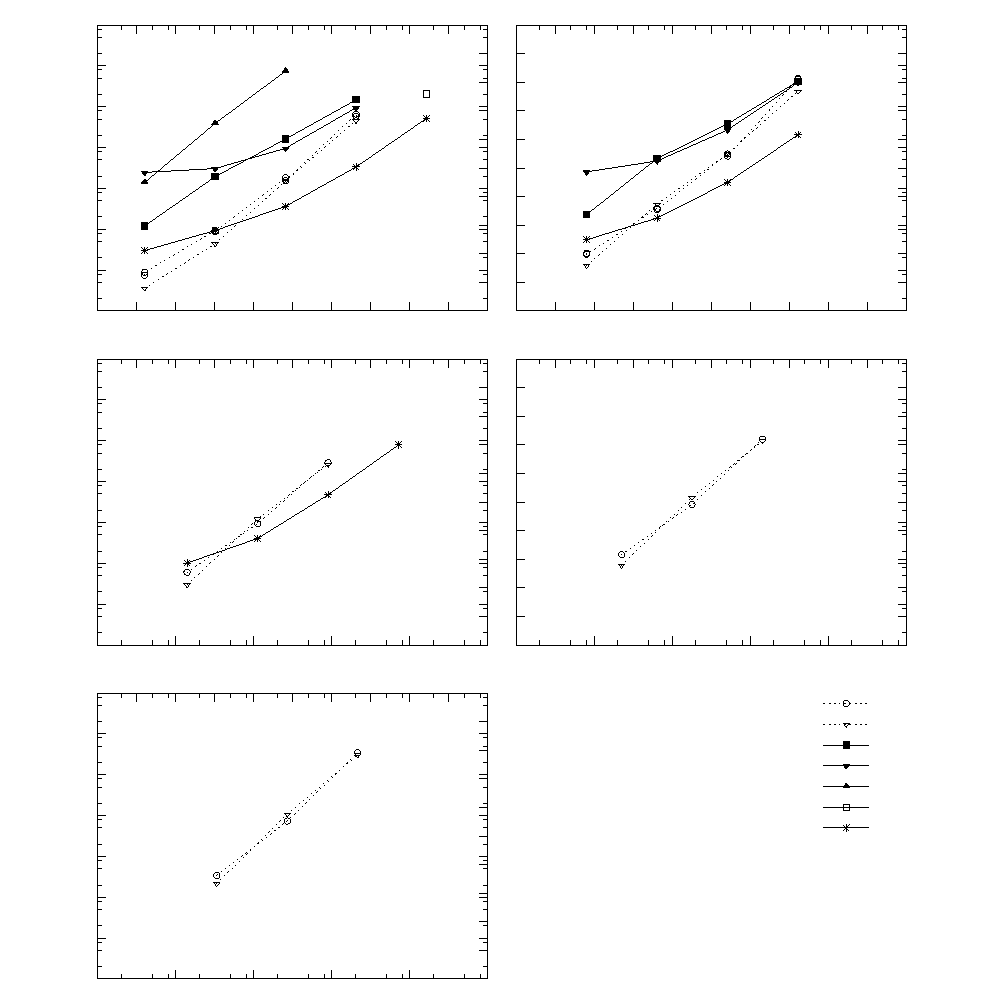
\includegraphics{ConstCoeffPoissonScaling}}%
    \gplfronttext
  \end{picture}%
\endgroup

	\end{center}
	\caption{
		Solver runtime vs. degrees-of-freedom, for different polynomial degrees $k$,
		for problem/Equation (\ref{eq:ContantCoeffPoissonBenchmark}).
	}
	\label{fig:ConstantCoeffRuntimes}
\end{figure}

\newpage

\subsubsection{Block Jacobian and Schwarz-Multigrid Preconditioning}

\begin{figure}[!h]
	\begin{center}
		\input{./apdx-NodeSolverPerformance/zeug/jacobischwarz-scheme.pdf_tex}
	\end{center}
	\caption{
		schematic of the Multigrid Schwarz \& Block Jacobian Preconditioning (for a CG solver).
	}
	\label{fig:schema_BlockPCG}
\end{figure}

\begin{figure}[!h]
	\begin{center}
		% GNUPLOT: LaTeX picture with Postscript
\begingroup
  \makeatletter
  \providecommand\color[2][]{%
    \GenericError{(gnuplot) \space\space\space\@spaces}{%
      Package color not loaded in conjunction with
      terminal option `colourtext'%
    }{See the gnuplot documentation for explanation.%
    }{Either use 'blacktext' in gnuplot or load the package
      color.sty in LaTeX.}%
    \renewcommand\color[2][]{}%
  }%
  \providecommand\includegraphics[2][]{%
    \GenericError{(gnuplot) \space\space\space\@spaces}{%
      Package graphicx or graphics not loaded%
    }{See the gnuplot documentation for explanation.%
    }{The gnuplot epslatex terminal needs graphicx.sty or graphics.sty.}%
    \renewcommand\includegraphics[2][]{}%
  }%
  \providecommand\rotatebox[2]{#2}%
  \@ifundefined{ifGPcolor}{%
    \newif\ifGPcolor
    \GPcolortrue
  }{}%
  \@ifundefined{ifGPblacktext}{%
    \newif\ifGPblacktext
    \GPblacktexttrue
  }{}%
  % define a \g@addto@macro without @ in the name:
  \let\gplgaddtomacro\g@addto@macro
  % define empty templates for all commands taking text:
  \gdef\gplbacktext{}%
  \gdef\gplfronttext{}%
  \makeatother
  \ifGPblacktext
    % no textcolor at all
    \def\colorrgb#1{}%
    \def\colorgray#1{}%
  \else
    % gray or color?
    \ifGPcolor
      \def\colorrgb#1{\color[rgb]{#1}}%
      \def\colorgray#1{\color[gray]{#1}}%
      \expandafter\def\csname LTw\endcsname{\color{white}}%
      \expandafter\def\csname LTb\endcsname{\color{black}}%
      \expandafter\def\csname LTa\endcsname{\color{black}}%
      \expandafter\def\csname LT0\endcsname{\color[rgb]{1,0,0}}%
      \expandafter\def\csname LT1\endcsname{\color[rgb]{0,1,0}}%
      \expandafter\def\csname LT2\endcsname{\color[rgb]{0,0,1}}%
      \expandafter\def\csname LT3\endcsname{\color[rgb]{1,0,1}}%
      \expandafter\def\csname LT4\endcsname{\color[rgb]{0,1,1}}%
      \expandafter\def\csname LT5\endcsname{\color[rgb]{1,1,0}}%
      \expandafter\def\csname LT6\endcsname{\color[rgb]{0,0,0}}%
      \expandafter\def\csname LT7\endcsname{\color[rgb]{1,0.3,0}}%
      \expandafter\def\csname LT8\endcsname{\color[rgb]{0.5,0.5,0.5}}%
    \else
      % gray
      \def\colorrgb#1{\color{black}}%
      \def\colorgray#1{\color[gray]{#1}}%
      \expandafter\def\csname LTw\endcsname{\color{white}}%
      \expandafter\def\csname LTb\endcsname{\color{black}}%
      \expandafter\def\csname LTa\endcsname{\color{black}}%
      \expandafter\def\csname LT0\endcsname{\color{black}}%
      \expandafter\def\csname LT1\endcsname{\color{black}}%
      \expandafter\def\csname LT2\endcsname{\color{black}}%
      \expandafter\def\csname LT3\endcsname{\color{black}}%
      \expandafter\def\csname LT4\endcsname{\color{black}}%
      \expandafter\def\csname LT5\endcsname{\color{black}}%
      \expandafter\def\csname LT6\endcsname{\color{black}}%
      \expandafter\def\csname LT7\endcsname{\color{black}}%
      \expandafter\def\csname LT8\endcsname{\color{black}}%
    \fi
  \fi
    \setlength{\unitlength}{0.0500bp}%
    \ifx\gptboxheight\undefined%
      \newlength{\gptboxheight}%
      \newlength{\gptboxwidth}%
      \newsavebox{\gptboxtext}%
    \fi%
    \setlength{\fboxrule}{0.5pt}%
    \setlength{\fboxsep}{1pt}%
\begin{picture}(7920.00,6800.00)%
    \gplgaddtomacro\gplbacktext{%
      \csname LTb\endcsname%
      \put(997,4735){\makebox(0,0)[r]{\strut{}$10^{-2}$}}%
      \csname LTb\endcsname%
      \put(997,5075){\makebox(0,0)[r]{\strut{}$10^{-1}$}}%
      \csname LTb\endcsname%
      \put(997,5415){\makebox(0,0)[r]{\strut{}$10^{0}$}}%
      \csname LTb\endcsname%
      \put(997,5755){\makebox(0,0)[r]{\strut{}$10^{1}$}}%
      \csname LTb\endcsname%
      \put(997,6096){\makebox(0,0)[r]{\strut{}$10^{2}$}}%
      \csname LTb\endcsname%
      \put(997,6436){\makebox(0,0)[r]{\strut{}$10^{3}$}}%
      \csname LTb\endcsname%
      \put(997,6776){\makebox(0,0)[r]{\strut{}$10^{4}$}}%
      \csname LTb\endcsname%
      \put(1099,4556){\makebox(0,0){\strut{} }}%
      \csname LTb\endcsname%
      \put(2137,4556){\makebox(0,0){\strut{} }}%
      \csname LTb\endcsname%
      \put(3176,4556){\makebox(0,0){\strut{} }}%
      \csname LTb\endcsname%
      \put(4214,4556){\makebox(0,0){\strut{} }}%
      \csname LTb\endcsname%
      \put(5252,4556){\makebox(0,0){\strut{} }}%
      \csname LTb\endcsname%
      \put(6291,4556){\makebox(0,0){\strut{} }}%
      \csname LTb\endcsname%
      \put(7329,4556){\makebox(0,0){\strut{} }}%
      \csname LTb\endcsname%
      \put(7431,4735){\makebox(0,0)[l]{\strut{} }}%
      \csname LTb\endcsname%
      \put(7431,5075){\makebox(0,0)[l]{\strut{} }}%
      \csname LTb\endcsname%
      \put(7431,5415){\makebox(0,0)[l]{\strut{} }}%
      \csname LTb\endcsname%
      \put(7431,5756){\makebox(0,0)[l]{\strut{} }}%
      \csname LTb\endcsname%
      \put(7431,6096){\makebox(0,0)[l]{\strut{} }}%
      \csname LTb\endcsname%
      \put(7431,6436){\makebox(0,0)[l]{\strut{} }}%
      \csname LTb\endcsname%
      \put(7431,6776){\makebox(0,0)[l]{\strut{} }}%
    }%
    \gplgaddtomacro\gplfronttext{%
      \csname LTb\endcsname%
      \put(397,5755){\rotatebox{-270}{\makebox(0,0){\strut{}$k = 2$}}}%
      \csname LTb\endcsname%
      \put(1884,6615){\makebox(0,0)[l]{\strut{}Slv Iter}}%
      \csname LTb\endcsname%
      \put(1884,6436){\makebox(0,0)[l]{\strut{}Slv Init}}%
      \csname LTb\endcsname%
      \put(1884,6257){\makebox(0,0)[l]{\strut{}Agg Init}}%
      \csname LTb\endcsname%
      \put(1884,6078){\makebox(0,0)[l]{\strut{}Mtx ass}}%
      \csname LTb\endcsname%
      \put(1884,5899){\makebox(0,0)[l]{\strut{}linear}}%
    }%
    \gplgaddtomacro\gplbacktext{%
      \csname LTb\endcsname%
      \put(997,2468){\makebox(0,0)[r]{\strut{}$10^{-2}$}}%
      \csname LTb\endcsname%
      \put(997,2808){\makebox(0,0)[r]{\strut{}$10^{-1}$}}%
      \csname LTb\endcsname%
      \put(997,3149){\makebox(0,0)[r]{\strut{}$10^{0}$}}%
      \csname LTb\endcsname%
      \put(997,3489){\makebox(0,0)[r]{\strut{}$10^{1}$}}%
      \csname LTb\endcsname%
      \put(997,3829){\makebox(0,0)[r]{\strut{}$10^{2}$}}%
      \csname LTb\endcsname%
      \put(997,4170){\makebox(0,0)[r]{\strut{}$10^{3}$}}%
      \csname LTb\endcsname%
      \put(997,4510){\makebox(0,0)[r]{\strut{}$10^{4}$}}%
      \csname LTb\endcsname%
      \put(1099,2289){\makebox(0,0){\strut{} }}%
      \csname LTb\endcsname%
      \put(2137,2289){\makebox(0,0){\strut{} }}%
      \csname LTb\endcsname%
      \put(3176,2289){\makebox(0,0){\strut{} }}%
      \csname LTb\endcsname%
      \put(4214,2289){\makebox(0,0){\strut{} }}%
      \csname LTb\endcsname%
      \put(5252,2289){\makebox(0,0){\strut{} }}%
      \csname LTb\endcsname%
      \put(6291,2289){\makebox(0,0){\strut{} }}%
      \csname LTb\endcsname%
      \put(7329,2289){\makebox(0,0){\strut{} }}%
      \csname LTb\endcsname%
      \put(7431,2468){\makebox(0,0)[l]{\strut{} }}%
      \csname LTb\endcsname%
      \put(7431,2808){\makebox(0,0)[l]{\strut{} }}%
      \csname LTb\endcsname%
      \put(7431,3149){\makebox(0,0)[l]{\strut{} }}%
      \csname LTb\endcsname%
      \put(7431,3489){\makebox(0,0)[l]{\strut{} }}%
      \csname LTb\endcsname%
      \put(7431,3829){\makebox(0,0)[l]{\strut{} }}%
      \csname LTb\endcsname%
      \put(7431,4170){\makebox(0,0)[l]{\strut{} }}%
      \csname LTb\endcsname%
      \put(7431,4510){\makebox(0,0)[l]{\strut{} }}%
      \csname LTb\endcsname%
      \put(1099,4689){\makebox(0,0){\strut{} }}%
      \csname LTb\endcsname%
      \put(2137,4689){\makebox(0,0){\strut{} }}%
      \csname LTb\endcsname%
      \put(3176,4689){\makebox(0,0){\strut{} }}%
      \csname LTb\endcsname%
      \put(4214,4689){\makebox(0,0){\strut{} }}%
      \csname LTb\endcsname%
      \put(5252,4689){\makebox(0,0){\strut{} }}%
      \csname LTb\endcsname%
      \put(6291,4689){\makebox(0,0){\strut{} }}%
      \csname LTb\endcsname%
      \put(7329,4689){\makebox(0,0){\strut{} }}%
    }%
    \gplgaddtomacro\gplfronttext{%
      \csname LTb\endcsname%
      \put(397,3489){\rotatebox{-270}{\makebox(0,0){\strut{}$k = 3$}}}%
    }%
    \gplgaddtomacro\gplbacktext{%
      \csname LTb\endcsname%
      \put(997,201){\makebox(0,0)[r]{\strut{}$10^{-2}$}}%
      \csname LTb\endcsname%
      \put(997,541){\makebox(0,0)[r]{\strut{}$10^{-1}$}}%
      \csname LTb\endcsname%
      \put(997,882){\makebox(0,0)[r]{\strut{}$10^{0}$}}%
      \csname LTb\endcsname%
      \put(997,1222){\makebox(0,0)[r]{\strut{}$10^{1}$}}%
      \csname LTb\endcsname%
      \put(997,1563){\makebox(0,0)[r]{\strut{}$10^{2}$}}%
      \csname LTb\endcsname%
      \put(997,1903){\makebox(0,0)[r]{\strut{}$10^{3}$}}%
      \csname LTb\endcsname%
      \put(997,2244){\makebox(0,0)[r]{\strut{}$10^{4}$}}%
      \csname LTb\endcsname%
      \put(1099,22){\makebox(0,0){\strut{}$10^{1}$}}%
      \csname LTb\endcsname%
      \put(2137,22){\makebox(0,0){\strut{}$10^{2}$}}%
      \csname LTb\endcsname%
      \put(3176,22){\makebox(0,0){\strut{}$10^{3}$}}%
      \csname LTb\endcsname%
      \put(4214,22){\makebox(0,0){\strut{}$10^{4}$}}%
      \csname LTb\endcsname%
      \put(5252,22){\makebox(0,0){\strut{}$10^{5}$}}%
      \csname LTb\endcsname%
      \put(6291,22){\makebox(0,0){\strut{}$10^{6}$}}%
      \csname LTb\endcsname%
      \put(7329,22){\makebox(0,0){\strut{}$10^{7}$}}%
      \csname LTb\endcsname%
      \put(7431,201){\makebox(0,0)[l]{\strut{} }}%
      \csname LTb\endcsname%
      \put(7431,542){\makebox(0,0)[l]{\strut{} }}%
      \csname LTb\endcsname%
      \put(7431,882){\makebox(0,0)[l]{\strut{} }}%
      \csname LTb\endcsname%
      \put(7431,1223){\makebox(0,0)[l]{\strut{} }}%
      \csname LTb\endcsname%
      \put(7431,1563){\makebox(0,0)[l]{\strut{} }}%
      \csname LTb\endcsname%
      \put(7431,1904){\makebox(0,0)[l]{\strut{} }}%
      \csname LTb\endcsname%
      \put(7431,2244){\makebox(0,0)[l]{\strut{} }}%
      \csname LTb\endcsname%
      \put(1099,2423){\makebox(0,0){\strut{} }}%
      \csname LTb\endcsname%
      \put(2137,2423){\makebox(0,0){\strut{} }}%
      \csname LTb\endcsname%
      \put(3176,2423){\makebox(0,0){\strut{} }}%
      \csname LTb\endcsname%
      \put(4214,2423){\makebox(0,0){\strut{} }}%
      \csname LTb\endcsname%
      \put(5252,2423){\makebox(0,0){\strut{} }}%
      \csname LTb\endcsname%
      \put(6291,2423){\makebox(0,0){\strut{} }}%
      \csname LTb\endcsname%
      \put(7329,2423){\makebox(0,0){\strut{} }}%
    }%
    \gplgaddtomacro\gplfronttext{%
      \csname LTb\endcsname%
      \put(397,1222){\rotatebox{-270}{\makebox(0,0){\strut{}$k = 5$}}}%
    }%
    \gplbacktext
    \put(0,0){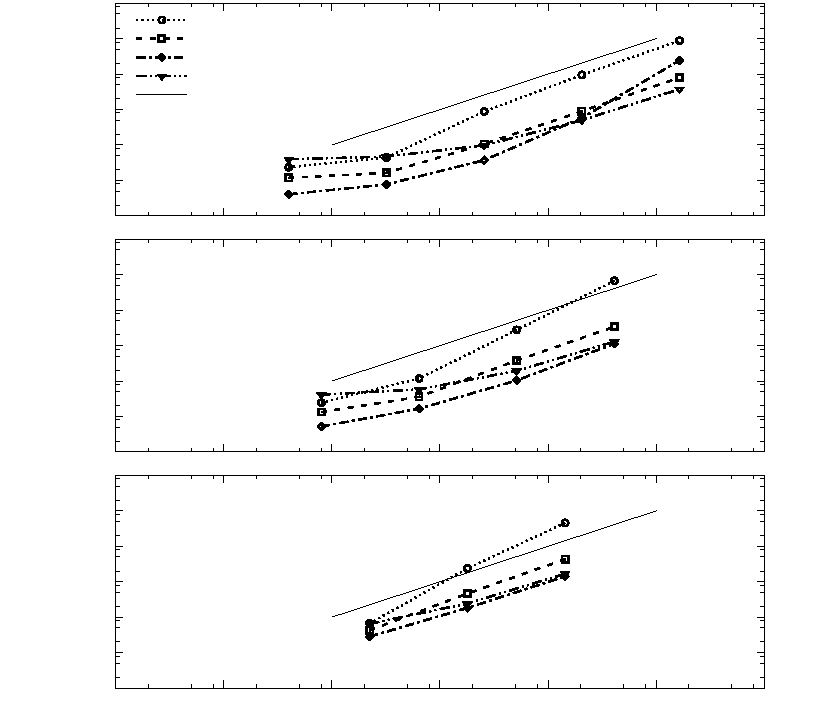
\includegraphics{ConstCoeffPoisson_MG}}%
    \gplfronttext
  \end{picture}%
\endgroup

	\end{center}
	\caption{
		Investigation of runtime of different code parts of the block Jacobian PCG. Solver runtime vs. degrees-of-freedom, for different polynomial degrees $k$,
		for problem/Equation (\ref{eq:ContantCoeffPoissonBenchmark}).
	}
	\label{fig:SIP_blockJacobianPCG}
\end{figure}
\newpage

\subsubsection{Schwarz-Multigrid Preconditioning}

\begin{figure}[!h]
	\begin{center}
		\input{./apdx-NodeSolverPerformance/zeug/schwarz-scheme.pdf_tex}
	\end{center}
	\caption{
		schematic of the Multigrid Schwarz \& Block Jacobian Preconditioning (for a CG solver).
	}
	\label{fig:schema_SchwarzPCG}
\end{figure}

\begin{figure}[!h]
	\begin{center}
		% GNUPLOT: LaTeX picture with Postscript
\begingroup
  \makeatletter
  \providecommand\color[2][]{%
    \GenericError{(gnuplot) \space\space\space\@spaces}{%
      Package color not loaded in conjunction with
      terminal option `colourtext'%
    }{See the gnuplot documentation for explanation.%
    }{Either use 'blacktext' in gnuplot or load the package
      color.sty in LaTeX.}%
    \renewcommand\color[2][]{}%
  }%
  \providecommand\includegraphics[2][]{%
    \GenericError{(gnuplot) \space\space\space\@spaces}{%
      Package graphicx or graphics not loaded%
    }{See the gnuplot documentation for explanation.%
    }{The gnuplot epslatex terminal needs graphicx.sty or graphics.sty.}%
    \renewcommand\includegraphics[2][]{}%
  }%
  \providecommand\rotatebox[2]{#2}%
  \@ifundefined{ifGPcolor}{%
    \newif\ifGPcolor
    \GPcolortrue
  }{}%
  \@ifundefined{ifGPblacktext}{%
    \newif\ifGPblacktext
    \GPblacktexttrue
  }{}%
  % define a \g@addto@macro without @ in the name:
  \let\gplgaddtomacro\g@addto@macro
  % define empty templates for all commands taking text:
  \gdef\gplbacktext{}%
  \gdef\gplfronttext{}%
  \makeatother
  \ifGPblacktext
    % no textcolor at all
    \def\colorrgb#1{}%
    \def\colorgray#1{}%
  \else
    % gray or color?
    \ifGPcolor
      \def\colorrgb#1{\color[rgb]{#1}}%
      \def\colorgray#1{\color[gray]{#1}}%
      \expandafter\def\csname LTw\endcsname{\color{white}}%
      \expandafter\def\csname LTb\endcsname{\color{black}}%
      \expandafter\def\csname LTa\endcsname{\color{black}}%
      \expandafter\def\csname LT0\endcsname{\color[rgb]{1,0,0}}%
      \expandafter\def\csname LT1\endcsname{\color[rgb]{0,1,0}}%
      \expandafter\def\csname LT2\endcsname{\color[rgb]{0,0,1}}%
      \expandafter\def\csname LT3\endcsname{\color[rgb]{1,0,1}}%
      \expandafter\def\csname LT4\endcsname{\color[rgb]{0,1,1}}%
      \expandafter\def\csname LT5\endcsname{\color[rgb]{1,1,0}}%
      \expandafter\def\csname LT6\endcsname{\color[rgb]{0,0,0}}%
      \expandafter\def\csname LT7\endcsname{\color[rgb]{1,0.3,0}}%
      \expandafter\def\csname LT8\endcsname{\color[rgb]{0.5,0.5,0.5}}%
    \else
      % gray
      \def\colorrgb#1{\color{black}}%
      \def\colorgray#1{\color[gray]{#1}}%
      \expandafter\def\csname LTw\endcsname{\color{white}}%
      \expandafter\def\csname LTb\endcsname{\color{black}}%
      \expandafter\def\csname LTa\endcsname{\color{black}}%
      \expandafter\def\csname LT0\endcsname{\color{black}}%
      \expandafter\def\csname LT1\endcsname{\color{black}}%
      \expandafter\def\csname LT2\endcsname{\color{black}}%
      \expandafter\def\csname LT3\endcsname{\color{black}}%
      \expandafter\def\csname LT4\endcsname{\color{black}}%
      \expandafter\def\csname LT5\endcsname{\color{black}}%
      \expandafter\def\csname LT6\endcsname{\color{black}}%
      \expandafter\def\csname LT7\endcsname{\color{black}}%
      \expandafter\def\csname LT8\endcsname{\color{black}}%
    \fi
  \fi
    \setlength{\unitlength}{0.0500bp}%
    \ifx\gptboxheight\undefined%
      \newlength{\gptboxheight}%
      \newlength{\gptboxwidth}%
      \newsavebox{\gptboxtext}%
    \fi%
    \setlength{\fboxrule}{0.5pt}%
    \setlength{\fboxsep}{1pt}%
\begin{picture}(9060.00,6800.00)%
    \gplgaddtomacro\gplbacktext{%
      \csname LTb\endcsname%
      \put(773,3831){\makebox(0,0)[r]{\strut{}$10^{-1}$}}%
      \csname LTb\endcsname%
      \put(773,4338){\makebox(0,0)[r]{\strut{}$10^{0}$}}%
      \csname LTb\endcsname%
      \put(773,4845){\makebox(0,0)[r]{\strut{}$10^{1}$}}%
      \csname LTb\endcsname%
      \put(773,5353){\makebox(0,0)[r]{\strut{}$10^{2}$}}%
      \csname LTb\endcsname%
      \put(773,5860){\makebox(0,0)[r]{\strut{}$10^{3}$}}%
      \csname LTb\endcsname%
      \put(773,6367){\makebox(0,0)[r]{\strut{}$10^{4}$}}%
      \csname LTb\endcsname%
      \put(861,3632){\makebox(0,0){\strut{}$10^{2}$}}%
      \csname LTb\endcsname%
      \put(2428,3632){\makebox(0,0){\strut{}$10^{3}$}}%
      \csname LTb\endcsname%
      \put(3995,3632){\makebox(0,0){\strut{}$10^{4}$}}%
      \csname LTb\endcsname%
      \put(5562,3632){\makebox(0,0){\strut{}$10^{5}$}}%
      \csname LTb\endcsname%
      \put(7129,3632){\makebox(0,0){\strut{}$10^{6}$}}%
      \csname LTb\endcsname%
      \put(7217,3831){\makebox(0,0)[l]{\strut{} }}%
      \csname LTb\endcsname%
      \put(7217,4338){\makebox(0,0)[l]{\strut{} }}%
      \csname LTb\endcsname%
      \put(7217,4845){\makebox(0,0)[l]{\strut{} }}%
      \csname LTb\endcsname%
      \put(7217,5353){\makebox(0,0)[l]{\strut{} }}%
      \csname LTb\endcsname%
      \put(7217,5860){\makebox(0,0)[l]{\strut{} }}%
      \csname LTb\endcsname%
      \put(7217,6367){\makebox(0,0)[l]{\strut{} }}%
      \csname LTb\endcsname%
      \put(861,6566){\makebox(0,0){\strut{} }}%
      \csname LTb\endcsname%
      \put(1756,6566){\makebox(0,0){\strut{} }}%
      \csname LTb\endcsname%
      \put(2652,6566){\makebox(0,0){\strut{} }}%
      \csname LTb\endcsname%
      \put(3547,6566){\makebox(0,0){\strut{} }}%
      \csname LTb\endcsname%
      \put(4443,6566){\makebox(0,0){\strut{} }}%
      \csname LTb\endcsname%
      \put(5338,6566){\makebox(0,0){\strut{} }}%
      \csname LTb\endcsname%
      \put(6234,6566){\makebox(0,0){\strut{} }}%
      \csname LTb\endcsname%
      \put(7129,6566){\makebox(0,0){\strut{} }}%
    }%
    \gplgaddtomacro\gplfronttext{%
      \csname LTb\endcsname%
      \put(233,5099){\rotatebox{-270}{\makebox(0,0){\strut{}$k = 2$}}}%
      \csname LTb\endcsname%
      \put(8273,6267){\makebox(0,0)[r]{\strut{}Slv Iter}}%
      \csname LTb\endcsname%
      \put(8273,6068){\makebox(0,0)[r]{\strut{}Slv Init}}%
      \csname LTb\endcsname%
      \put(8273,5869){\makebox(0,0)[r]{\strut{}Agg Init}}%
      \csname LTb\endcsname%
      \put(8273,5670){\makebox(0,0)[r]{\strut{}Mtx ass}}%
      \csname LTb\endcsname%
      \put(8273,5471){\makebox(0,0)[r]{\strut{}linear}}%
    }%
    \gplgaddtomacro\gplbacktext{%
      \csname LTb\endcsname%
      \put(773,431){\makebox(0,0)[r]{\strut{}$10^{-1}$}}%
      \csname LTb\endcsname%
      \put(773,938){\makebox(0,0)[r]{\strut{}$10^{0}$}}%
      \csname LTb\endcsname%
      \put(773,1446){\makebox(0,0)[r]{\strut{}$10^{1}$}}%
      \csname LTb\endcsname%
      \put(773,1953){\makebox(0,0)[r]{\strut{}$10^{2}$}}%
      \csname LTb\endcsname%
      \put(773,2461){\makebox(0,0)[r]{\strut{}$10^{3}$}}%
      \csname LTb\endcsname%
      \put(773,2968){\makebox(0,0)[r]{\strut{}$10^{4}$}}%
      \csname LTb\endcsname%
      \put(861,232){\makebox(0,0){\strut{}$10^{2}$}}%
      \csname LTb\endcsname%
      \put(2428,232){\makebox(0,0){\strut{}$10^{3}$}}%
      \csname LTb\endcsname%
      \put(3995,232){\makebox(0,0){\strut{}$10^{4}$}}%
      \csname LTb\endcsname%
      \put(5562,232){\makebox(0,0){\strut{}$10^{5}$}}%
      \csname LTb\endcsname%
      \put(7129,232){\makebox(0,0){\strut{}$10^{6}$}}%
      \csname LTb\endcsname%
      \put(7217,431){\makebox(0,0)[l]{\strut{} }}%
      \csname LTb\endcsname%
      \put(7217,938){\makebox(0,0)[l]{\strut{} }}%
      \csname LTb\endcsname%
      \put(7217,1446){\makebox(0,0)[l]{\strut{} }}%
      \csname LTb\endcsname%
      \put(7217,1953){\makebox(0,0)[l]{\strut{} }}%
      \csname LTb\endcsname%
      \put(7217,2461){\makebox(0,0)[l]{\strut{} }}%
      \csname LTb\endcsname%
      \put(7217,2968){\makebox(0,0)[l]{\strut{} }}%
      \csname LTb\endcsname%
      \put(861,3167){\makebox(0,0){\strut{} }}%
      \csname LTb\endcsname%
      \put(1756,3167){\makebox(0,0){\strut{} }}%
      \csname LTb\endcsname%
      \put(2652,3167){\makebox(0,0){\strut{} }}%
      \csname LTb\endcsname%
      \put(3547,3167){\makebox(0,0){\strut{} }}%
      \csname LTb\endcsname%
      \put(4443,3167){\makebox(0,0){\strut{} }}%
      \csname LTb\endcsname%
      \put(5338,3167){\makebox(0,0){\strut{} }}%
      \csname LTb\endcsname%
      \put(6234,3167){\makebox(0,0){\strut{} }}%
      \csname LTb\endcsname%
      \put(7129,3167){\makebox(0,0){\strut{} }}%
    }%
    \gplgaddtomacro\gplfronttext{%
      \csname LTb\endcsname%
      \put(233,1699){\rotatebox{-270}{\makebox(0,0){\strut{}$k = 3$}}}%
      \csname LTb\endcsname%
      \put(8273,2868){\makebox(0,0)[r]{\strut{}Slv Iter}}%
      \csname LTb\endcsname%
      \put(8273,2669){\makebox(0,0)[r]{\strut{}Slv Init}}%
      \csname LTb\endcsname%
      \put(8273,2470){\makebox(0,0)[r]{\strut{}Agg Init}}%
      \csname LTb\endcsname%
      \put(8273,2271){\makebox(0,0)[r]{\strut{}Mtx ass}}%
      \csname LTb\endcsname%
      \put(8273,2072){\makebox(0,0)[r]{\strut{}linear}}%
    }%
    \gplbacktext
    \put(0,0){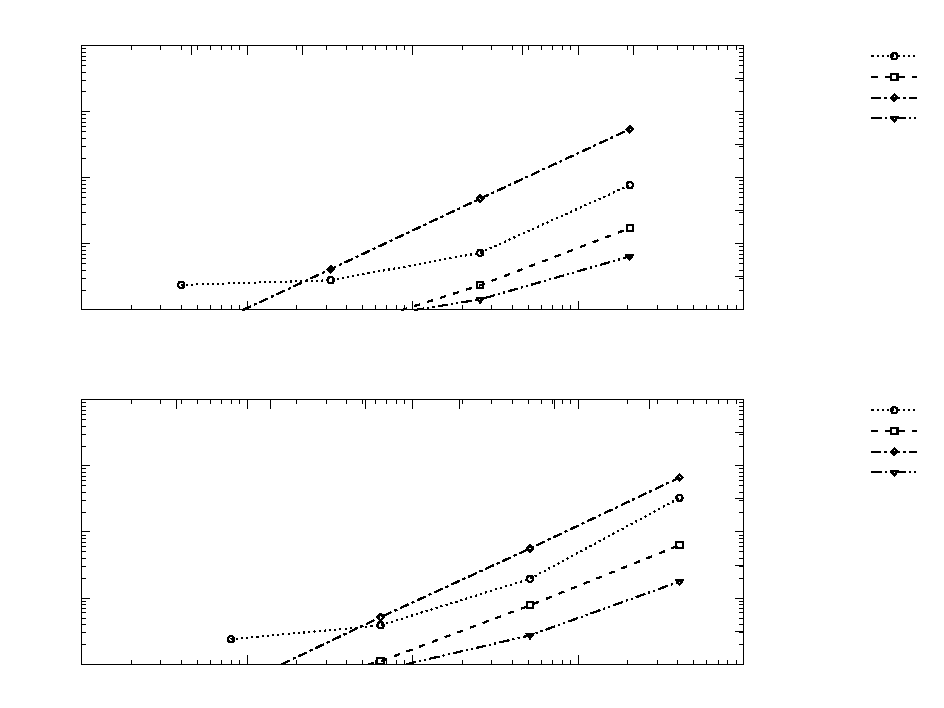
\includegraphics{ConstCoeffPoisson_Schwarz}}%
    \gplfronttext
  \end{picture}%
\endgroup

	\end{center}
	\caption{
		Investigation of runtime of different code parts of the Schwarz PCG. Solver runtime vs. degrees-of-freedom, for different polynomial degrees $k$,
		for problem/Equation (\ref{eq:ContantCoeffPoissonBenchmark}).
	}
	\label{fig:SIP_SchwarzPGC}
\end{figure}
\newpage

\subsection{velocity test problem with levelset and Xdg}
\label{sec:XdgPoisson}
The problem
\begin{equation}
\left\{ \begin{array} {rclll}
- \nabla \cdot (\mu \nabla \vec{u})   & = & g_{\domain}=(1, 1, 1)^T                       
& \text{in}\ \Omega \setminus \varphi, \text{with}\ \Omega= [-1,1]^3  &  \\
% ----
\vec{u_D} & = & (0, 0, 0)^T                             
& \text{on}\ \Gamma_D = \partial \Omega
& \text{Dirichlet-boundary} \\
% ----
\jump{\mu \nabla \vec{u}} \cdot \vec{n} & = & (0, 0, 0)^T  & \text{on}\ \varphi = \{\vec{X}=(x,y,z); \ |\vec{X}|_2=0.7\} & \text{levelset}
\end{array} \right.
\label{eq:XdgPoissonBenchmark}
\end{equation}
where $\mu_1=1$ (inner) and $\mu_2=1000$ (outer) characterize the two phases. is investigated on a uniform, equidistant Cartesian grid. See \ref{fig:XdgRuntimes} for results.

\graphicspath{{./apdx-NodeSolverPerformance/XDGPoisson/plots/}}

\begin{figure}[!h]
	\begin{center}
		% GNUPLOT: LaTeX picture with Postscript
\begingroup
  \makeatletter
  \providecommand\color[2][]{%
    \GenericError{(gnuplot) \space\space\space\@spaces}{%
      Package color not loaded in conjunction with
      terminal option `colourtext'%
    }{See the gnuplot documentation for explanation.%
    }{Either use 'blacktext' in gnuplot or load the package
      color.sty in LaTeX.}%
    \renewcommand\color[2][]{}%
  }%
  \providecommand\includegraphics[2][]{%
    \GenericError{(gnuplot) \space\space\space\@spaces}{%
      Package graphicx or graphics not loaded%
    }{See the gnuplot documentation for explanation.%
    }{The gnuplot epslatex terminal needs graphicx.sty or graphics.sty.}%
    \renewcommand\includegraphics[2][]{}%
  }%
  \providecommand\rotatebox[2]{#2}%
  \@ifundefined{ifGPcolor}{%
    \newif\ifGPcolor
    \GPcolortrue
  }{}%
  \@ifundefined{ifGPblacktext}{%
    \newif\ifGPblacktext
    \GPblacktexttrue
  }{}%
  % define a \g@addto@macro without @ in the name:
  \let\gplgaddtomacro\g@addto@macro
  % define empty templates for all commands taking text:
  \gdef\gplbacktext{}%
  \gdef\gplfronttext{}%
  \makeatother
  \ifGPblacktext
    % no textcolor at all
    \def\colorrgb#1{}%
    \def\colorgray#1{}%
  \else
    % gray or color?
    \ifGPcolor
      \def\colorrgb#1{\color[rgb]{#1}}%
      \def\colorgray#1{\color[gray]{#1}}%
      \expandafter\def\csname LTw\endcsname{\color{white}}%
      \expandafter\def\csname LTb\endcsname{\color{black}}%
      \expandafter\def\csname LTa\endcsname{\color{black}}%
      \expandafter\def\csname LT0\endcsname{\color[rgb]{1,0,0}}%
      \expandafter\def\csname LT1\endcsname{\color[rgb]{0,1,0}}%
      \expandafter\def\csname LT2\endcsname{\color[rgb]{0,0,1}}%
      \expandafter\def\csname LT3\endcsname{\color[rgb]{1,0,1}}%
      \expandafter\def\csname LT4\endcsname{\color[rgb]{0,1,1}}%
      \expandafter\def\csname LT5\endcsname{\color[rgb]{1,1,0}}%
      \expandafter\def\csname LT6\endcsname{\color[rgb]{0,0,0}}%
      \expandafter\def\csname LT7\endcsname{\color[rgb]{1,0.3,0}}%
      \expandafter\def\csname LT8\endcsname{\color[rgb]{0.5,0.5,0.5}}%
    \else
      % gray
      \def\colorrgb#1{\color{black}}%
      \def\colorgray#1{\color[gray]{#1}}%
      \expandafter\def\csname LTw\endcsname{\color{white}}%
      \expandafter\def\csname LTb\endcsname{\color{black}}%
      \expandafter\def\csname LTa\endcsname{\color{black}}%
      \expandafter\def\csname LT0\endcsname{\color{black}}%
      \expandafter\def\csname LT1\endcsname{\color{black}}%
      \expandafter\def\csname LT2\endcsname{\color{black}}%
      \expandafter\def\csname LT3\endcsname{\color{black}}%
      \expandafter\def\csname LT4\endcsname{\color{black}}%
      \expandafter\def\csname LT5\endcsname{\color{black}}%
      \expandafter\def\csname LT6\endcsname{\color{black}}%
      \expandafter\def\csname LT7\endcsname{\color{black}}%
      \expandafter\def\csname LT8\endcsname{\color{black}}%
    \fi
  \fi
    \setlength{\unitlength}{0.0500bp}%
    \ifx\gptboxheight\undefined%
      \newlength{\gptboxheight}%
      \newlength{\gptboxwidth}%
      \newsavebox{\gptboxtext}%
    \fi%
    \setlength{\fboxrule}{0.5pt}%
    \setlength{\fboxsep}{1pt}%
\begin{picture}(7920.00,6800.00)%
    \gplgaddtomacro\gplbacktext{%
      \csname LTb\endcsname%
      \put(997,4735){\makebox(0,0)[r]{\strut{}$10^{-1}$}}%
      \csname LTb\endcsname%
      \put(997,5075){\makebox(0,0)[r]{\strut{}$10^{0}$}}%
      \csname LTb\endcsname%
      \put(997,5415){\makebox(0,0)[r]{\strut{}$10^{1}$}}%
      \csname LTb\endcsname%
      \put(997,5755){\makebox(0,0)[r]{\strut{}$10^{2}$}}%
      \csname LTb\endcsname%
      \put(997,6096){\makebox(0,0)[r]{\strut{}$10^{3}$}}%
      \csname LTb\endcsname%
      \put(997,6436){\makebox(0,0)[r]{\strut{}$10^{4}$}}%
      \csname LTb\endcsname%
      \put(997,6776){\makebox(0,0)[r]{\strut{}$10^{5}$}}%
      \csname LTb\endcsname%
      \put(1099,4556){\makebox(0,0){\strut{} }}%
      \csname LTb\endcsname%
      \put(2137,4556){\makebox(0,0){\strut{} }}%
      \csname LTb\endcsname%
      \put(3176,4556){\makebox(0,0){\strut{} }}%
      \csname LTb\endcsname%
      \put(4214,4556){\makebox(0,0){\strut{} }}%
      \csname LTb\endcsname%
      \put(5252,4556){\makebox(0,0){\strut{} }}%
      \csname LTb\endcsname%
      \put(6291,4556){\makebox(0,0){\strut{} }}%
      \csname LTb\endcsname%
      \put(7329,4556){\makebox(0,0){\strut{} }}%
      \csname LTb\endcsname%
      \put(7431,4735){\makebox(0,0)[l]{\strut{} }}%
      \csname LTb\endcsname%
      \put(7431,5075){\makebox(0,0)[l]{\strut{} }}%
      \csname LTb\endcsname%
      \put(7431,5415){\makebox(0,0)[l]{\strut{} }}%
      \csname LTb\endcsname%
      \put(7431,5756){\makebox(0,0)[l]{\strut{} }}%
      \csname LTb\endcsname%
      \put(7431,6096){\makebox(0,0)[l]{\strut{} }}%
      \csname LTb\endcsname%
      \put(7431,6436){\makebox(0,0)[l]{\strut{} }}%
      \csname LTb\endcsname%
      \put(7431,6776){\makebox(0,0)[l]{\strut{} }}%
    }%
    \gplgaddtomacro\gplfronttext{%
      \csname LTb\endcsname%
      \put(397,5755){\rotatebox{-270}{\makebox(0,0){\strut{}$k = 2$}}}%
      \csname LTb\endcsname%
      \put(2190,6565){\makebox(0,0)[l]{\strut{}Pardiso}}%
      \csname LTb\endcsname%
      \put(2190,6286){\makebox(0,0)[l]{\strut{}GMRES w. pTG}}%
      \csname LTb\endcsname%
      \put(2190,6007){\makebox(0,0)[l]{\strut{}Kcycle w. add.-Schwarz}}%
      \csname LTb\endcsname%
      \put(2190,5728){\makebox(0,0)[l]{\strut{}linear}}%
    }%
    \gplgaddtomacro\gplbacktext{%
      \csname LTb\endcsname%
      \put(997,2468){\makebox(0,0)[r]{\strut{}$10^{-1}$}}%
      \csname LTb\endcsname%
      \put(997,2808){\makebox(0,0)[r]{\strut{}$10^{0}$}}%
      \csname LTb\endcsname%
      \put(997,3149){\makebox(0,0)[r]{\strut{}$10^{1}$}}%
      \csname LTb\endcsname%
      \put(997,3489){\makebox(0,0)[r]{\strut{}$10^{2}$}}%
      \csname LTb\endcsname%
      \put(997,3829){\makebox(0,0)[r]{\strut{}$10^{3}$}}%
      \csname LTb\endcsname%
      \put(997,4170){\makebox(0,0)[r]{\strut{}$10^{4}$}}%
      \csname LTb\endcsname%
      \put(997,4510){\makebox(0,0)[r]{\strut{}$10^{5}$}}%
      \csname LTb\endcsname%
      \put(1099,2289){\makebox(0,0){\strut{} }}%
      \csname LTb\endcsname%
      \put(2137,2289){\makebox(0,0){\strut{} }}%
      \csname LTb\endcsname%
      \put(3176,2289){\makebox(0,0){\strut{} }}%
      \csname LTb\endcsname%
      \put(4214,2289){\makebox(0,0){\strut{} }}%
      \csname LTb\endcsname%
      \put(5252,2289){\makebox(0,0){\strut{} }}%
      \csname LTb\endcsname%
      \put(6291,2289){\makebox(0,0){\strut{} }}%
      \csname LTb\endcsname%
      \put(7329,2289){\makebox(0,0){\strut{} }}%
      \csname LTb\endcsname%
      \put(7431,2468){\makebox(0,0)[l]{\strut{} }}%
      \csname LTb\endcsname%
      \put(7431,2808){\makebox(0,0)[l]{\strut{} }}%
      \csname LTb\endcsname%
      \put(7431,3149){\makebox(0,0)[l]{\strut{} }}%
      \csname LTb\endcsname%
      \put(7431,3489){\makebox(0,0)[l]{\strut{} }}%
      \csname LTb\endcsname%
      \put(7431,3829){\makebox(0,0)[l]{\strut{} }}%
      \csname LTb\endcsname%
      \put(7431,4170){\makebox(0,0)[l]{\strut{} }}%
      \csname LTb\endcsname%
      \put(7431,4510){\makebox(0,0)[l]{\strut{} }}%
      \csname LTb\endcsname%
      \put(1099,4689){\makebox(0,0){\strut{} }}%
      \csname LTb\endcsname%
      \put(2137,4689){\makebox(0,0){\strut{} }}%
      \csname LTb\endcsname%
      \put(3176,4689){\makebox(0,0){\strut{} }}%
      \csname LTb\endcsname%
      \put(4214,4689){\makebox(0,0){\strut{} }}%
      \csname LTb\endcsname%
      \put(5252,4689){\makebox(0,0){\strut{} }}%
      \csname LTb\endcsname%
      \put(6291,4689){\makebox(0,0){\strut{} }}%
      \csname LTb\endcsname%
      \put(7329,4689){\makebox(0,0){\strut{} }}%
    }%
    \gplgaddtomacro\gplfronttext{%
      \csname LTb\endcsname%
      \put(397,3489){\rotatebox{-270}{\makebox(0,0){\strut{}$k = 3$}}}%
    }%
    \gplgaddtomacro\gplbacktext{%
      \csname LTb\endcsname%
      \put(997,201){\makebox(0,0)[r]{\strut{}$10^{-1}$}}%
      \csname LTb\endcsname%
      \put(997,541){\makebox(0,0)[r]{\strut{}$10^{0}$}}%
      \csname LTb\endcsname%
      \put(997,882){\makebox(0,0)[r]{\strut{}$10^{1}$}}%
      \csname LTb\endcsname%
      \put(997,1222){\makebox(0,0)[r]{\strut{}$10^{2}$}}%
      \csname LTb\endcsname%
      \put(997,1563){\makebox(0,0)[r]{\strut{}$10^{3}$}}%
      \csname LTb\endcsname%
      \put(997,1903){\makebox(0,0)[r]{\strut{}$10^{4}$}}%
      \csname LTb\endcsname%
      \put(997,2244){\makebox(0,0)[r]{\strut{}$10^{5}$}}%
      \csname LTb\endcsname%
      \put(7431,201){\makebox(0,0)[l]{\strut{} }}%
      \csname LTb\endcsname%
      \put(7431,542){\makebox(0,0)[l]{\strut{} }}%
      \csname LTb\endcsname%
      \put(7431,882){\makebox(0,0)[l]{\strut{} }}%
      \csname LTb\endcsname%
      \put(7431,1223){\makebox(0,0)[l]{\strut{} }}%
      \csname LTb\endcsname%
      \put(7431,1563){\makebox(0,0)[l]{\strut{} }}%
      \csname LTb\endcsname%
      \put(7431,1904){\makebox(0,0)[l]{\strut{} }}%
      \csname LTb\endcsname%
      \put(7431,2244){\makebox(0,0)[l]{\strut{} }}%
      \csname LTb\endcsname%
      \put(1099,2423){\makebox(0,0){\strut{} }}%
      \csname LTb\endcsname%
      \put(2137,2423){\makebox(0,0){\strut{} }}%
      \csname LTb\endcsname%
      \put(3176,2423){\makebox(0,0){\strut{} }}%
      \csname LTb\endcsname%
      \put(4214,2423){\makebox(0,0){\strut{} }}%
      \csname LTb\endcsname%
      \put(5252,2423){\makebox(0,0){\strut{} }}%
      \csname LTb\endcsname%
      \put(6291,2423){\makebox(0,0){\strut{} }}%
      \csname LTb\endcsname%
      \put(7329,2423){\makebox(0,0){\strut{} }}%
    }%
    \gplgaddtomacro\gplfronttext{%
      \csname LTb\endcsname%
      \put(397,1222){\rotatebox{-270}{\makebox(0,0){\strut{}$k = 5$}}}%
    }%
    \gplbacktext
    \put(0,0){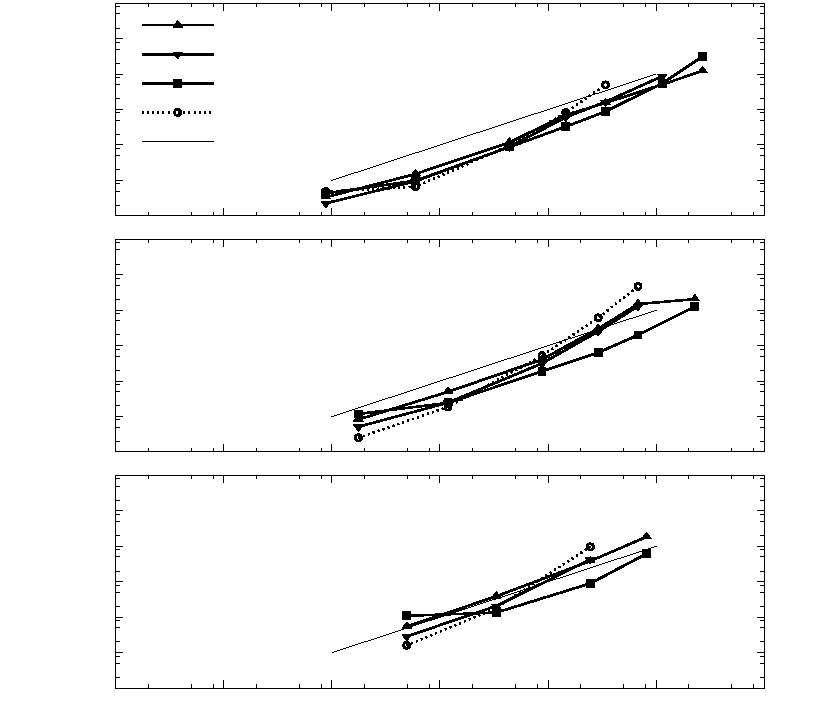
\includegraphics{XdgPoissonScaling}}%
    \gplfronttext
  \end{picture}%
\endgroup

	\end{center}
	\caption{
		Solver runtime vs. degrees-of-freedom, for different polynomial degrees $k$,
		for problem/Equation (\ref{eq:XdgPoissonBenchmark}).
	}
	\label{fig:XdgRuntimes}
\end{figure}
\newpage
Subsequent the performance of some code parts are investigated for the block Jacobian and the Schwarz multigrid preconditioned conjugate gradient method (PCG):
\begin{itemize}
	\item MatrixAssembly: assemble Block matrix
	\item Aggregation basis init: create multigrid sequence, contains information about the transformation at the multigrid levels
	\item Solver Init: hand over/assemble relevant data for the chosen solver, e.g. operator matrix etc.
	\item Solver Run: solves the equation system: operator matrix, vector of dg coordinates and given RHS 
\end{itemize}
Both variants are using pre and post smoothing solvers (5 runs at each multigrid level).

\subsubsection{Block Jacobian and Schwarz-Multigrid Preconditioning}

\begin{figure}[!h]
	\begin{center}
		\input{./apdx-NodeSolverPerformance/zeug/jacobischwarz-scheme.pdf_tex}
	\end{center}
	\caption{
		schematic of the Multigrid Schwarz \& Block Jacobian Preconditioning (for a CG solver).
	}
	\label{fig:schema_BlockPCG_2}
\end{figure}

\begin{figure}[!h]
	\begin{center}
		% GNUPLOT: LaTeX picture with Postscript
\begingroup
  \makeatletter
  \providecommand\color[2][]{%
    \GenericError{(gnuplot) \space\space\space\@spaces}{%
      Package color not loaded in conjunction with
      terminal option `colourtext'%
    }{See the gnuplot documentation for explanation.%
    }{Either use 'blacktext' in gnuplot or load the package
      color.sty in LaTeX.}%
    \renewcommand\color[2][]{}%
  }%
  \providecommand\includegraphics[2][]{%
    \GenericError{(gnuplot) \space\space\space\@spaces}{%
      Package graphicx or graphics not loaded%
    }{See the gnuplot documentation for explanation.%
    }{The gnuplot epslatex terminal needs graphicx.sty or graphics.sty.}%
    \renewcommand\includegraphics[2][]{}%
  }%
  \providecommand\rotatebox[2]{#2}%
  \@ifundefined{ifGPcolor}{%
    \newif\ifGPcolor
    \GPcolortrue
  }{}%
  \@ifundefined{ifGPblacktext}{%
    \newif\ifGPblacktext
    \GPblacktexttrue
  }{}%
  % define a \g@addto@macro without @ in the name:
  \let\gplgaddtomacro\g@addto@macro
  % define empty templates for all commands taking text:
  \gdef\gplbacktext{}%
  \gdef\gplfronttext{}%
  \makeatother
  \ifGPblacktext
    % no textcolor at all
    \def\colorrgb#1{}%
    \def\colorgray#1{}%
  \else
    % gray or color?
    \ifGPcolor
      \def\colorrgb#1{\color[rgb]{#1}}%
      \def\colorgray#1{\color[gray]{#1}}%
      \expandafter\def\csname LTw\endcsname{\color{white}}%
      \expandafter\def\csname LTb\endcsname{\color{black}}%
      \expandafter\def\csname LTa\endcsname{\color{black}}%
      \expandafter\def\csname LT0\endcsname{\color[rgb]{1,0,0}}%
      \expandafter\def\csname LT1\endcsname{\color[rgb]{0,1,0}}%
      \expandafter\def\csname LT2\endcsname{\color[rgb]{0,0,1}}%
      \expandafter\def\csname LT3\endcsname{\color[rgb]{1,0,1}}%
      \expandafter\def\csname LT4\endcsname{\color[rgb]{0,1,1}}%
      \expandafter\def\csname LT5\endcsname{\color[rgb]{1,1,0}}%
      \expandafter\def\csname LT6\endcsname{\color[rgb]{0,0,0}}%
      \expandafter\def\csname LT7\endcsname{\color[rgb]{1,0.3,0}}%
      \expandafter\def\csname LT8\endcsname{\color[rgb]{0.5,0.5,0.5}}%
    \else
      % gray
      \def\colorrgb#1{\color{black}}%
      \def\colorgray#1{\color[gray]{#1}}%
      \expandafter\def\csname LTw\endcsname{\color{white}}%
      \expandafter\def\csname LTb\endcsname{\color{black}}%
      \expandafter\def\csname LTa\endcsname{\color{black}}%
      \expandafter\def\csname LT0\endcsname{\color{black}}%
      \expandafter\def\csname LT1\endcsname{\color{black}}%
      \expandafter\def\csname LT2\endcsname{\color{black}}%
      \expandafter\def\csname LT3\endcsname{\color{black}}%
      \expandafter\def\csname LT4\endcsname{\color{black}}%
      \expandafter\def\csname LT5\endcsname{\color{black}}%
      \expandafter\def\csname LT6\endcsname{\color{black}}%
      \expandafter\def\csname LT7\endcsname{\color{black}}%
      \expandafter\def\csname LT8\endcsname{\color{black}}%
    \fi
  \fi
    \setlength{\unitlength}{0.0500bp}%
    \ifx\gptboxheight\undefined%
      \newlength{\gptboxheight}%
      \newlength{\gptboxwidth}%
      \newsavebox{\gptboxtext}%
    \fi%
    \setlength{\fboxrule}{0.5pt}%
    \setlength{\fboxsep}{1pt}%
\begin{picture}(7920.00,6800.00)%
    \gplgaddtomacro\gplbacktext{%
      \csname LTb\endcsname%
      \put(997,4735){\makebox(0,0)[r]{\strut{}$10^{-2}$}}%
      \csname LTb\endcsname%
      \put(997,5075){\makebox(0,0)[r]{\strut{}$10^{-1}$}}%
      \csname LTb\endcsname%
      \put(997,5415){\makebox(0,0)[r]{\strut{}$10^{0}$}}%
      \csname LTb\endcsname%
      \put(997,5755){\makebox(0,0)[r]{\strut{}$10^{1}$}}%
      \csname LTb\endcsname%
      \put(997,6096){\makebox(0,0)[r]{\strut{}$10^{2}$}}%
      \csname LTb\endcsname%
      \put(997,6436){\makebox(0,0)[r]{\strut{}$10^{3}$}}%
      \csname LTb\endcsname%
      \put(997,6776){\makebox(0,0)[r]{\strut{}$10^{4}$}}%
      \csname LTb\endcsname%
      \put(1099,4556){\makebox(0,0){\strut{} }}%
      \csname LTb\endcsname%
      \put(2137,4556){\makebox(0,0){\strut{} }}%
      \csname LTb\endcsname%
      \put(3176,4556){\makebox(0,0){\strut{} }}%
      \csname LTb\endcsname%
      \put(4214,4556){\makebox(0,0){\strut{} }}%
      \csname LTb\endcsname%
      \put(5252,4556){\makebox(0,0){\strut{} }}%
      \csname LTb\endcsname%
      \put(6291,4556){\makebox(0,0){\strut{} }}%
      \csname LTb\endcsname%
      \put(7329,4556){\makebox(0,0){\strut{} }}%
      \csname LTb\endcsname%
      \put(7431,4735){\makebox(0,0)[l]{\strut{} }}%
      \csname LTb\endcsname%
      \put(7431,5075){\makebox(0,0)[l]{\strut{} }}%
      \csname LTb\endcsname%
      \put(7431,5415){\makebox(0,0)[l]{\strut{} }}%
      \csname LTb\endcsname%
      \put(7431,5756){\makebox(0,0)[l]{\strut{} }}%
      \csname LTb\endcsname%
      \put(7431,6096){\makebox(0,0)[l]{\strut{} }}%
      \csname LTb\endcsname%
      \put(7431,6436){\makebox(0,0)[l]{\strut{} }}%
      \csname LTb\endcsname%
      \put(7431,6776){\makebox(0,0)[l]{\strut{} }}%
    }%
    \gplgaddtomacro\gplfronttext{%
      \csname LTb\endcsname%
      \put(397,5755){\rotatebox{-270}{\makebox(0,0){\strut{}$k = 2$}}}%
      \csname LTb\endcsname%
      \put(1884,6615){\makebox(0,0)[l]{\strut{}Slv Iter}}%
      \csname LTb\endcsname%
      \put(1884,6436){\makebox(0,0)[l]{\strut{}Slv Init}}%
      \csname LTb\endcsname%
      \put(1884,6257){\makebox(0,0)[l]{\strut{}Agg Init}}%
      \csname LTb\endcsname%
      \put(1884,6078){\makebox(0,0)[l]{\strut{}Mtx ass}}%
      \csname LTb\endcsname%
      \put(1884,5899){\makebox(0,0)[l]{\strut{}linear}}%
    }%
    \gplgaddtomacro\gplbacktext{%
      \csname LTb\endcsname%
      \put(997,2468){\makebox(0,0)[r]{\strut{}$10^{-2}$}}%
      \csname LTb\endcsname%
      \put(997,2808){\makebox(0,0)[r]{\strut{}$10^{-1}$}}%
      \csname LTb\endcsname%
      \put(997,3149){\makebox(0,0)[r]{\strut{}$10^{0}$}}%
      \csname LTb\endcsname%
      \put(997,3489){\makebox(0,0)[r]{\strut{}$10^{1}$}}%
      \csname LTb\endcsname%
      \put(997,3829){\makebox(0,0)[r]{\strut{}$10^{2}$}}%
      \csname LTb\endcsname%
      \put(997,4170){\makebox(0,0)[r]{\strut{}$10^{3}$}}%
      \csname LTb\endcsname%
      \put(997,4510){\makebox(0,0)[r]{\strut{}$10^{4}$}}%
      \csname LTb\endcsname%
      \put(1099,2289){\makebox(0,0){\strut{} }}%
      \csname LTb\endcsname%
      \put(2137,2289){\makebox(0,0){\strut{} }}%
      \csname LTb\endcsname%
      \put(3176,2289){\makebox(0,0){\strut{} }}%
      \csname LTb\endcsname%
      \put(4214,2289){\makebox(0,0){\strut{} }}%
      \csname LTb\endcsname%
      \put(5252,2289){\makebox(0,0){\strut{} }}%
      \csname LTb\endcsname%
      \put(6291,2289){\makebox(0,0){\strut{} }}%
      \csname LTb\endcsname%
      \put(7329,2289){\makebox(0,0){\strut{} }}%
      \csname LTb\endcsname%
      \put(7431,2468){\makebox(0,0)[l]{\strut{} }}%
      \csname LTb\endcsname%
      \put(7431,2808){\makebox(0,0)[l]{\strut{} }}%
      \csname LTb\endcsname%
      \put(7431,3149){\makebox(0,0)[l]{\strut{} }}%
      \csname LTb\endcsname%
      \put(7431,3489){\makebox(0,0)[l]{\strut{} }}%
      \csname LTb\endcsname%
      \put(7431,3829){\makebox(0,0)[l]{\strut{} }}%
      \csname LTb\endcsname%
      \put(7431,4170){\makebox(0,0)[l]{\strut{} }}%
      \csname LTb\endcsname%
      \put(7431,4510){\makebox(0,0)[l]{\strut{} }}%
      \csname LTb\endcsname%
      \put(1099,4689){\makebox(0,0){\strut{} }}%
      \csname LTb\endcsname%
      \put(2137,4689){\makebox(0,0){\strut{} }}%
      \csname LTb\endcsname%
      \put(3176,4689){\makebox(0,0){\strut{} }}%
      \csname LTb\endcsname%
      \put(4214,4689){\makebox(0,0){\strut{} }}%
      \csname LTb\endcsname%
      \put(5252,4689){\makebox(0,0){\strut{} }}%
      \csname LTb\endcsname%
      \put(6291,4689){\makebox(0,0){\strut{} }}%
      \csname LTb\endcsname%
      \put(7329,4689){\makebox(0,0){\strut{} }}%
    }%
    \gplgaddtomacro\gplfronttext{%
      \csname LTb\endcsname%
      \put(397,3489){\rotatebox{-270}{\makebox(0,0){\strut{}$k = 3$}}}%
    }%
    \gplgaddtomacro\gplbacktext{%
      \csname LTb\endcsname%
      \put(997,201){\makebox(0,0)[r]{\strut{}$10^{-2}$}}%
      \csname LTb\endcsname%
      \put(997,541){\makebox(0,0)[r]{\strut{}$10^{-1}$}}%
      \csname LTb\endcsname%
      \put(997,882){\makebox(0,0)[r]{\strut{}$10^{0}$}}%
      \csname LTb\endcsname%
      \put(997,1222){\makebox(0,0)[r]{\strut{}$10^{1}$}}%
      \csname LTb\endcsname%
      \put(997,1563){\makebox(0,0)[r]{\strut{}$10^{2}$}}%
      \csname LTb\endcsname%
      \put(997,1903){\makebox(0,0)[r]{\strut{}$10^{3}$}}%
      \csname LTb\endcsname%
      \put(997,2244){\makebox(0,0)[r]{\strut{}$10^{4}$}}%
      \csname LTb\endcsname%
      \put(1099,22){\makebox(0,0){\strut{}$10^{1}$}}%
      \csname LTb\endcsname%
      \put(2137,22){\makebox(0,0){\strut{}$10^{2}$}}%
      \csname LTb\endcsname%
      \put(3176,22){\makebox(0,0){\strut{}$10^{3}$}}%
      \csname LTb\endcsname%
      \put(4214,22){\makebox(0,0){\strut{}$10^{4}$}}%
      \csname LTb\endcsname%
      \put(5252,22){\makebox(0,0){\strut{}$10^{5}$}}%
      \csname LTb\endcsname%
      \put(6291,22){\makebox(0,0){\strut{}$10^{6}$}}%
      \csname LTb\endcsname%
      \put(7329,22){\makebox(0,0){\strut{}$10^{7}$}}%
      \csname LTb\endcsname%
      \put(7431,201){\makebox(0,0)[l]{\strut{} }}%
      \csname LTb\endcsname%
      \put(7431,542){\makebox(0,0)[l]{\strut{} }}%
      \csname LTb\endcsname%
      \put(7431,882){\makebox(0,0)[l]{\strut{} }}%
      \csname LTb\endcsname%
      \put(7431,1223){\makebox(0,0)[l]{\strut{} }}%
      \csname LTb\endcsname%
      \put(7431,1563){\makebox(0,0)[l]{\strut{} }}%
      \csname LTb\endcsname%
      \put(7431,1904){\makebox(0,0)[l]{\strut{} }}%
      \csname LTb\endcsname%
      \put(7431,2244){\makebox(0,0)[l]{\strut{} }}%
      \csname LTb\endcsname%
      \put(1099,2423){\makebox(0,0){\strut{} }}%
      \csname LTb\endcsname%
      \put(2137,2423){\makebox(0,0){\strut{} }}%
      \csname LTb\endcsname%
      \put(3176,2423){\makebox(0,0){\strut{} }}%
      \csname LTb\endcsname%
      \put(4214,2423){\makebox(0,0){\strut{} }}%
      \csname LTb\endcsname%
      \put(5252,2423){\makebox(0,0){\strut{} }}%
      \csname LTb\endcsname%
      \put(6291,2423){\makebox(0,0){\strut{} }}%
      \csname LTb\endcsname%
      \put(7329,2423){\makebox(0,0){\strut{} }}%
    }%
    \gplgaddtomacro\gplfronttext{%
      \csname LTb\endcsname%
      \put(397,1222){\rotatebox{-270}{\makebox(0,0){\strut{}$k = 5$}}}%
    }%
    \gplbacktext
    \put(0,0){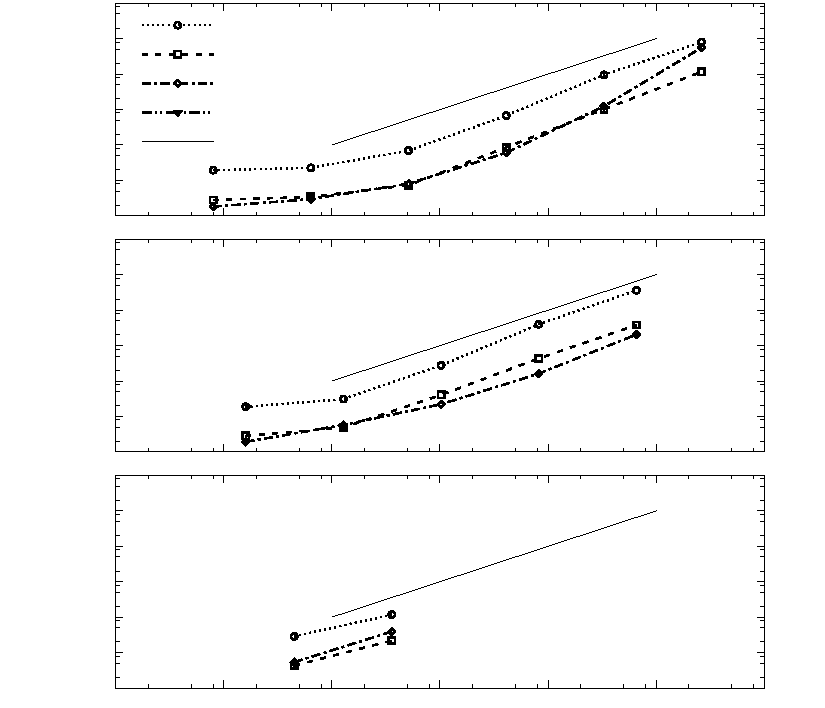
\includegraphics{XdgPoisson_MG}}%
    \gplfronttext
  \end{picture}%
\endgroup

	\end{center}
	\caption{
		Investigation of runtime of different code parts of the block Jacobian PCG. Solver runtime vs. degrees-of-freedom, for different polynomial degrees $k$,
		for problem/Equation (\ref{eq:XdgPoissonBenchmark}).
	}
	\label{fig:Xdg_blockJacobianPCG}
\end{figure}

\subsubsection{Schwarz-Multigrid Preconditioning}

\begin{figure}[!h]
	\begin{center}
		\input{./apdx-NodeSolverPerformance/zeug/schwarz-scheme.pdf_tex}
	\end{center}
	\caption{
		schematic of the Multigrid Schwarz \& Block Jacobian Preconditioning (for a CG solver).
	}
	\label{fig:schema_SchwarzPCG_2}
\end{figure}

\newpage
\begin{figure}[!h]
	\begin{center}
		% GNUPLOT: LaTeX picture with Postscript
\begingroup
  \makeatletter
  \providecommand\color[2][]{%
    \GenericError{(gnuplot) \space\space\space\@spaces}{%
      Package color not loaded in conjunction with
      terminal option `colourtext'%
    }{See the gnuplot documentation for explanation.%
    }{Either use 'blacktext' in gnuplot or load the package
      color.sty in LaTeX.}%
    \renewcommand\color[2][]{}%
  }%
  \providecommand\includegraphics[2][]{%
    \GenericError{(gnuplot) \space\space\space\@spaces}{%
      Package graphicx or graphics not loaded%
    }{See the gnuplot documentation for explanation.%
    }{The gnuplot epslatex terminal needs graphicx.sty or graphics.sty.}%
    \renewcommand\includegraphics[2][]{}%
  }%
  \providecommand\rotatebox[2]{#2}%
  \@ifundefined{ifGPcolor}{%
    \newif\ifGPcolor
    \GPcolortrue
  }{}%
  \@ifundefined{ifGPblacktext}{%
    \newif\ifGPblacktext
    \GPblacktexttrue
  }{}%
  % define a \g@addto@macro without @ in the name:
  \let\gplgaddtomacro\g@addto@macro
  % define empty templates for all commands taking text:
  \gdef\gplbacktext{}%
  \gdef\gplfronttext{}%
  \makeatother
  \ifGPblacktext
    % no textcolor at all
    \def\colorrgb#1{}%
    \def\colorgray#1{}%
  \else
    % gray or color?
    \ifGPcolor
      \def\colorrgb#1{\color[rgb]{#1}}%
      \def\colorgray#1{\color[gray]{#1}}%
      \expandafter\def\csname LTw\endcsname{\color{white}}%
      \expandafter\def\csname LTb\endcsname{\color{black}}%
      \expandafter\def\csname LTa\endcsname{\color{black}}%
      \expandafter\def\csname LT0\endcsname{\color[rgb]{1,0,0}}%
      \expandafter\def\csname LT1\endcsname{\color[rgb]{0,1,0}}%
      \expandafter\def\csname LT2\endcsname{\color[rgb]{0,0,1}}%
      \expandafter\def\csname LT3\endcsname{\color[rgb]{1,0,1}}%
      \expandafter\def\csname LT4\endcsname{\color[rgb]{0,1,1}}%
      \expandafter\def\csname LT5\endcsname{\color[rgb]{1,1,0}}%
      \expandafter\def\csname LT6\endcsname{\color[rgb]{0,0,0}}%
      \expandafter\def\csname LT7\endcsname{\color[rgb]{1,0.3,0}}%
      \expandafter\def\csname LT8\endcsname{\color[rgb]{0.5,0.5,0.5}}%
    \else
      % gray
      \def\colorrgb#1{\color{black}}%
      \def\colorgray#1{\color[gray]{#1}}%
      \expandafter\def\csname LTw\endcsname{\color{white}}%
      \expandafter\def\csname LTb\endcsname{\color{black}}%
      \expandafter\def\csname LTa\endcsname{\color{black}}%
      \expandafter\def\csname LT0\endcsname{\color{black}}%
      \expandafter\def\csname LT1\endcsname{\color{black}}%
      \expandafter\def\csname LT2\endcsname{\color{black}}%
      \expandafter\def\csname LT3\endcsname{\color{black}}%
      \expandafter\def\csname LT4\endcsname{\color{black}}%
      \expandafter\def\csname LT5\endcsname{\color{black}}%
      \expandafter\def\csname LT6\endcsname{\color{black}}%
      \expandafter\def\csname LT7\endcsname{\color{black}}%
      \expandafter\def\csname LT8\endcsname{\color{black}}%
    \fi
  \fi
    \setlength{\unitlength}{0.0500bp}%
    \ifx\gptboxheight\undefined%
      \newlength{\gptboxheight}%
      \newlength{\gptboxwidth}%
      \newsavebox{\gptboxtext}%
    \fi%
    \setlength{\fboxrule}{0.5pt}%
    \setlength{\fboxsep}{1pt}%
\begin{picture}(7920.00,6800.00)%
    \gplgaddtomacro\gplbacktext{%
      \csname LTb\endcsname%
      \put(997,4735){\makebox(0,0)[r]{\strut{}$10^{-2}$}}%
      \csname LTb\endcsname%
      \put(997,5075){\makebox(0,0)[r]{\strut{}$10^{-1}$}}%
      \csname LTb\endcsname%
      \put(997,5415){\makebox(0,0)[r]{\strut{}$10^{0}$}}%
      \csname LTb\endcsname%
      \put(997,5755){\makebox(0,0)[r]{\strut{}$10^{1}$}}%
      \csname LTb\endcsname%
      \put(997,6096){\makebox(0,0)[r]{\strut{}$10^{2}$}}%
      \csname LTb\endcsname%
      \put(997,6436){\makebox(0,0)[r]{\strut{}$10^{3}$}}%
      \csname LTb\endcsname%
      \put(997,6776){\makebox(0,0)[r]{\strut{}$10^{4}$}}%
      \csname LTb\endcsname%
      \put(1099,4556){\makebox(0,0){\strut{} }}%
      \csname LTb\endcsname%
      \put(2137,4556){\makebox(0,0){\strut{} }}%
      \csname LTb\endcsname%
      \put(3176,4556){\makebox(0,0){\strut{} }}%
      \csname LTb\endcsname%
      \put(4214,4556){\makebox(0,0){\strut{} }}%
      \csname LTb\endcsname%
      \put(5252,4556){\makebox(0,0){\strut{} }}%
      \csname LTb\endcsname%
      \put(6291,4556){\makebox(0,0){\strut{} }}%
      \csname LTb\endcsname%
      \put(7329,4556){\makebox(0,0){\strut{} }}%
      \csname LTb\endcsname%
      \put(7431,4735){\makebox(0,0)[l]{\strut{} }}%
      \csname LTb\endcsname%
      \put(7431,5075){\makebox(0,0)[l]{\strut{} }}%
      \csname LTb\endcsname%
      \put(7431,5415){\makebox(0,0)[l]{\strut{} }}%
      \csname LTb\endcsname%
      \put(7431,5756){\makebox(0,0)[l]{\strut{} }}%
      \csname LTb\endcsname%
      \put(7431,6096){\makebox(0,0)[l]{\strut{} }}%
      \csname LTb\endcsname%
      \put(7431,6436){\makebox(0,0)[l]{\strut{} }}%
      \csname LTb\endcsname%
      \put(7431,6776){\makebox(0,0)[l]{\strut{} }}%
    }%
    \gplgaddtomacro\gplfronttext{%
      \csname LTb\endcsname%
      \put(397,5755){\rotatebox{-270}{\makebox(0,0){\strut{}$k = 2$}}}%
      \csname LTb\endcsname%
      \put(2190,6565){\makebox(0,0)[l]{\strut{}Slv Iter}}%
      \csname LTb\endcsname%
      \put(2190,6286){\makebox(0,0)[l]{\strut{}Slv Init}}%
      \csname LTb\endcsname%
      \put(2190,6007){\makebox(0,0)[l]{\strut{}Agg Init}}%
      \csname LTb\endcsname%
      \put(2190,5728){\makebox(0,0)[l]{\strut{}Mtx ass}}%
      \csname LTb\endcsname%
      \put(2190,5449){\makebox(0,0)[l]{\strut{}linear}}%
    }%
    \gplgaddtomacro\gplbacktext{%
      \csname LTb\endcsname%
      \put(997,2468){\makebox(0,0)[r]{\strut{}$10^{-2}$}}%
      \csname LTb\endcsname%
      \put(997,2808){\makebox(0,0)[r]{\strut{}$10^{-1}$}}%
      \csname LTb\endcsname%
      \put(997,3149){\makebox(0,0)[r]{\strut{}$10^{0}$}}%
      \csname LTb\endcsname%
      \put(997,3489){\makebox(0,0)[r]{\strut{}$10^{1}$}}%
      \csname LTb\endcsname%
      \put(997,3829){\makebox(0,0)[r]{\strut{}$10^{2}$}}%
      \csname LTb\endcsname%
      \put(997,4170){\makebox(0,0)[r]{\strut{}$10^{3}$}}%
      \csname LTb\endcsname%
      \put(997,4510){\makebox(0,0)[r]{\strut{}$10^{4}$}}%
      \csname LTb\endcsname%
      \put(1099,2289){\makebox(0,0){\strut{} }}%
      \csname LTb\endcsname%
      \put(2137,2289){\makebox(0,0){\strut{} }}%
      \csname LTb\endcsname%
      \put(3176,2289){\makebox(0,0){\strut{} }}%
      \csname LTb\endcsname%
      \put(4214,2289){\makebox(0,0){\strut{} }}%
      \csname LTb\endcsname%
      \put(5252,2289){\makebox(0,0){\strut{} }}%
      \csname LTb\endcsname%
      \put(6291,2289){\makebox(0,0){\strut{} }}%
      \csname LTb\endcsname%
      \put(7329,2289){\makebox(0,0){\strut{} }}%
      \csname LTb\endcsname%
      \put(7431,2468){\makebox(0,0)[l]{\strut{} }}%
      \csname LTb\endcsname%
      \put(7431,2808){\makebox(0,0)[l]{\strut{} }}%
      \csname LTb\endcsname%
      \put(7431,3149){\makebox(0,0)[l]{\strut{} }}%
      \csname LTb\endcsname%
      \put(7431,3489){\makebox(0,0)[l]{\strut{} }}%
      \csname LTb\endcsname%
      \put(7431,3829){\makebox(0,0)[l]{\strut{} }}%
      \csname LTb\endcsname%
      \put(7431,4170){\makebox(0,0)[l]{\strut{} }}%
      \csname LTb\endcsname%
      \put(7431,4510){\makebox(0,0)[l]{\strut{} }}%
      \csname LTb\endcsname%
      \put(1099,4689){\makebox(0,0){\strut{} }}%
      \csname LTb\endcsname%
      \put(2137,4689){\makebox(0,0){\strut{} }}%
      \csname LTb\endcsname%
      \put(3176,4689){\makebox(0,0){\strut{} }}%
      \csname LTb\endcsname%
      \put(4214,4689){\makebox(0,0){\strut{} }}%
      \csname LTb\endcsname%
      \put(5252,4689){\makebox(0,0){\strut{} }}%
      \csname LTb\endcsname%
      \put(6291,4689){\makebox(0,0){\strut{} }}%
      \csname LTb\endcsname%
      \put(7329,4689){\makebox(0,0){\strut{} }}%
    }%
    \gplgaddtomacro\gplfronttext{%
      \csname LTb\endcsname%
      \put(397,3489){\rotatebox{-270}{\makebox(0,0){\strut{}$k = 3$}}}%
    }%
    \gplgaddtomacro\gplbacktext{%
      \csname LTb\endcsname%
      \put(997,201){\makebox(0,0)[r]{\strut{}$10^{-2}$}}%
      \csname LTb\endcsname%
      \put(997,541){\makebox(0,0)[r]{\strut{}$10^{-1}$}}%
      \csname LTb\endcsname%
      \put(997,882){\makebox(0,0)[r]{\strut{}$10^{0}$}}%
      \csname LTb\endcsname%
      \put(997,1222){\makebox(0,0)[r]{\strut{}$10^{1}$}}%
      \csname LTb\endcsname%
      \put(997,1563){\makebox(0,0)[r]{\strut{}$10^{2}$}}%
      \csname LTb\endcsname%
      \put(997,1903){\makebox(0,0)[r]{\strut{}$10^{3}$}}%
      \csname LTb\endcsname%
      \put(997,2244){\makebox(0,0)[r]{\strut{}$10^{4}$}}%
      \csname LTb\endcsname%
      \put(7431,201){\makebox(0,0)[l]{\strut{} }}%
      \csname LTb\endcsname%
      \put(7431,542){\makebox(0,0)[l]{\strut{} }}%
      \csname LTb\endcsname%
      \put(7431,882){\makebox(0,0)[l]{\strut{} }}%
      \csname LTb\endcsname%
      \put(7431,1223){\makebox(0,0)[l]{\strut{} }}%
      \csname LTb\endcsname%
      \put(7431,1563){\makebox(0,0)[l]{\strut{} }}%
      \csname LTb\endcsname%
      \put(7431,1904){\makebox(0,0)[l]{\strut{} }}%
      \csname LTb\endcsname%
      \put(7431,2244){\makebox(0,0)[l]{\strut{} }}%
      \csname LTb\endcsname%
      \put(1099,2423){\makebox(0,0){\strut{} }}%
      \csname LTb\endcsname%
      \put(2137,2423){\makebox(0,0){\strut{} }}%
      \csname LTb\endcsname%
      \put(3176,2423){\makebox(0,0){\strut{} }}%
      \csname LTb\endcsname%
      \put(4214,2423){\makebox(0,0){\strut{} }}%
      \csname LTb\endcsname%
      \put(5252,2423){\makebox(0,0){\strut{} }}%
      \csname LTb\endcsname%
      \put(6291,2423){\makebox(0,0){\strut{} }}%
      \csname LTb\endcsname%
      \put(7329,2423){\makebox(0,0){\strut{} }}%
    }%
    \gplgaddtomacro\gplfronttext{%
      \csname LTb\endcsname%
      \put(397,1222){\rotatebox{-270}{\makebox(0,0){\strut{}$k = 5$}}}%
    }%
    \gplbacktext
    \put(0,0){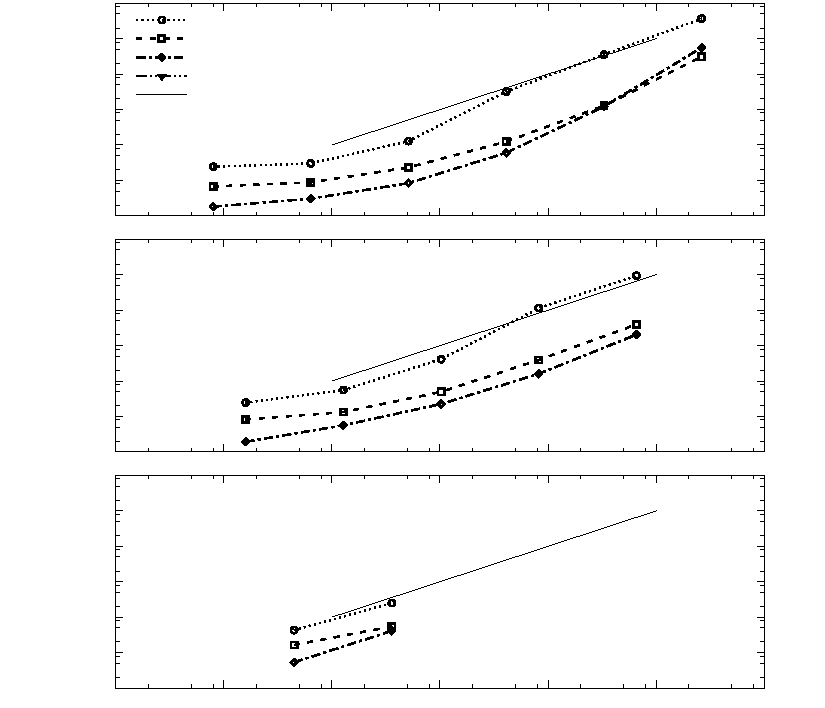
\includegraphics{XdgPoisson_Schwarz}}%
    \gplfronttext
  \end{picture}%
\endgroup

	\end{center}
	\caption{
		Investigation of runtime of different code parts of the Schwarz PCG. Solver runtime vs. degrees-of-freedom, for different polynomial degrees $k$,
		for problem/Equation (\ref{eq:XdgPoissonBenchmark}).
	}
	\label{fig:Xdg_SchwarzPGC}
\end{figure}
\newpage


\section{Solver Performance - Navier-Stokes problems}
\label{sec:SolverPerformanceNSE}
Different solver strategies are conducted to solve the fully coupled incompressible Navier-Stokes equations. At the moment the following strategies can be examined:
\begin{itemize}
	\item Linearizsation of the NSE with: Newton(Gmres) or Picard
	\item Solving the linear problem with a Gmres approach or the direct solver MUMPS
	\item Preconditioning with Additive-Schwarz domain decomposition (with coarse solve on the coarsest multigrid level) and direct solver MUMPS for the Blocks (Automatic)
	\item Preconditioning with Additive-Schwarz kcycle Blocks on the coarsest multigrid level (with coarse solve on the coarsest multigrid level) and direct solver MUMPS for the Blocks
\end{itemize}
\subsection{Driven Cavity 3D}
The problem
\begin{equation}
\left\{ \begin{array} {rclll}
\rho_f\Big(\frac{\partial \vec{u}}{\partial t}+ \vec{u} \cdot \nabla \vec{u}\Big) +\nabla p - \mu_f \Delta \vec{u} & = & \vec{f}
& \text{and}\   &  \\
% ----
\nabla \cdot \vec{u} & = & 0
& \text{in}\ \Omega = (-0.5,0.5) \times (-0.5,0.5) \times (-0.5,0.5)  & \\
\vec{u}_D & = & \{1,0,0 \}
& \text{on}\ \Gamma_D = \{ (x,y,0z) \in \real^3; \ z = 0.5 \}
& \text{Dirichlet-boundary}\\
\vec{u}_W & = & 0
& \text{on}\ \Gamma_W = \partial \Omega \setminus \Gamma_D
& \text{Dirichlet-boundary}\\
\vec{u}_0(x,y,z) & = & \{1,0,0\}
& \text{in}\ \Omega = (-0.5,0.5) \times (-0.5,0.5) \times (-0.5,0.5)
& \text{Initial Condition}
\end{array} \right.
\label{eq:NavierStokesCavityBenchmark}
\end{equation}
is investigated on different cartesian grids. The physical parameters of the fluid are choosen to be $\rho_f=1$ and $\mu_f=0.0025$ which renders down to a Reynoldsnumber of 400.

\graphicspath{{./apdx-NodeSolverPerformance/NavierStokesDrivenCavity/plots/}}

\begin{figure}[h!]
	\begin{center}
		% GNUPLOT: LaTeX picture with Postscript
\begingroup
  \makeatletter
  \providecommand\color[2][]{%
    \GenericError{(gnuplot) \space\space\space\@spaces}{%
      Package color not loaded in conjunction with
      terminal option `colourtext'%
    }{See the gnuplot documentation for explanation.%
    }{Either use 'blacktext' in gnuplot or load the package
      color.sty in LaTeX.}%
    \renewcommand\color[2][]{}%
  }%
  \providecommand\includegraphics[2][]{%
    \GenericError{(gnuplot) \space\space\space\@spaces}{%
      Package graphicx or graphics not loaded%
    }{See the gnuplot documentation for explanation.%
    }{The gnuplot epslatex terminal needs graphicx.sty or graphics.sty.}%
    \renewcommand\includegraphics[2][]{}%
  }%
  \providecommand\rotatebox[2]{#2}%
  \@ifundefined{ifGPcolor}{%
    \newif\ifGPcolor
    \GPcolortrue
  }{}%
  \@ifundefined{ifGPblacktext}{%
    \newif\ifGPblacktext
    \GPblacktexttrue
  }{}%
  % define a \g@addto@macro without @ in the name:
  \let\gplgaddtomacro\g@addto@macro
  % define empty templates for all commands taking text:
  \gdef\gplbacktext{}%
  \gdef\gplfronttext{}%
  \makeatother
  \ifGPblacktext
    % no textcolor at all
    \def\colorrgb#1{}%
    \def\colorgray#1{}%
  \else
    % gray or color?
    \ifGPcolor
      \def\colorrgb#1{\color[rgb]{#1}}%
      \def\colorgray#1{\color[gray]{#1}}%
      \expandafter\def\csname LTw\endcsname{\color{white}}%
      \expandafter\def\csname LTb\endcsname{\color{black}}%
      \expandafter\def\csname LTa\endcsname{\color{black}}%
      \expandafter\def\csname LT0\endcsname{\color[rgb]{1,0,0}}%
      \expandafter\def\csname LT1\endcsname{\color[rgb]{0,1,0}}%
      \expandafter\def\csname LT2\endcsname{\color[rgb]{0,0,1}}%
      \expandafter\def\csname LT3\endcsname{\color[rgb]{1,0,1}}%
      \expandafter\def\csname LT4\endcsname{\color[rgb]{0,1,1}}%
      \expandafter\def\csname LT5\endcsname{\color[rgb]{1,1,0}}%
      \expandafter\def\csname LT6\endcsname{\color[rgb]{0,0,0}}%
      \expandafter\def\csname LT7\endcsname{\color[rgb]{1,0.3,0}}%
      \expandafter\def\csname LT8\endcsname{\color[rgb]{0.5,0.5,0.5}}%
    \else
      % gray
      \def\colorrgb#1{\color{black}}%
      \def\colorgray#1{\color[gray]{#1}}%
      \expandafter\def\csname LTw\endcsname{\color{white}}%
      \expandafter\def\csname LTb\endcsname{\color{black}}%
      \expandafter\def\csname LTa\endcsname{\color{black}}%
      \expandafter\def\csname LT0\endcsname{\color{black}}%
      \expandafter\def\csname LT1\endcsname{\color{black}}%
      \expandafter\def\csname LT2\endcsname{\color{black}}%
      \expandafter\def\csname LT3\endcsname{\color{black}}%
      \expandafter\def\csname LT4\endcsname{\color{black}}%
      \expandafter\def\csname LT5\endcsname{\color{black}}%
      \expandafter\def\csname LT6\endcsname{\color{black}}%
      \expandafter\def\csname LT7\endcsname{\color{black}}%
      \expandafter\def\csname LT8\endcsname{\color{black}}%
    \fi
  \fi
    \setlength{\unitlength}{0.0500bp}%
    \ifx\gptboxheight\undefined%
      \newlength{\gptboxheight}%
      \newlength{\gptboxwidth}%
      \newsavebox{\gptboxtext}%
    \fi%
    \setlength{\fboxrule}{0.5pt}%
    \setlength{\fboxsep}{1pt}%
\begin{picture}(12460.00,5660.00)%
    \gplgaddtomacro\gplbacktext{%
      \csname LTb\endcsname%
      \put(762,772){\makebox(0,0)[r]{\strut{}$10^{1}$}}%
      \csname LTb\endcsname%
      \put(762,1801){\makebox(0,0)[r]{\strut{}$10^{2}$}}%
      \csname LTb\endcsname%
      \put(762,2829){\makebox(0,0)[r]{\strut{}$10^{3}$}}%
      \csname LTb\endcsname%
      \put(762,3858){\makebox(0,0)[r]{\strut{}$10^{4}$}}%
      \csname LTb\endcsname%
      \put(762,4886){\makebox(0,0)[r]{\strut{}$10^{5}$}}%
      \csname LTb\endcsname%
      \put(864,593){\makebox(0,0){\strut{}$10^{3}$}}%
      \csname LTb\endcsname%
      \put(2420,593){\makebox(0,0){\strut{}$10^{4}$}}%
      \csname LTb\endcsname%
      \put(3975,593){\makebox(0,0){\strut{}$10^{5}$}}%
      \csname LTb\endcsname%
      \put(5531,593){\makebox(0,0){\strut{}$10^{6}$}}%
      \csname LTb\endcsname%
      \put(5633,772){\makebox(0,0)[l]{\strut{} }}%
      \csname LTb\endcsname%
      \put(5633,1286){\makebox(0,0)[l]{\strut{} }}%
      \csname LTb\endcsname%
      \put(5633,1801){\makebox(0,0)[l]{\strut{} }}%
      \csname LTb\endcsname%
      \put(5633,2315){\makebox(0,0)[l]{\strut{} }}%
      \csname LTb\endcsname%
      \put(5633,2829){\makebox(0,0)[l]{\strut{} }}%
      \csname LTb\endcsname%
      \put(5633,3343){\makebox(0,0)[l]{\strut{} }}%
      \csname LTb\endcsname%
      \put(5633,3858){\makebox(0,0)[l]{\strut{} }}%
      \csname LTb\endcsname%
      \put(5633,4372){\makebox(0,0)[l]{\strut{} }}%
      \csname LTb\endcsname%
      \put(5633,4886){\makebox(0,0)[l]{\strut{} }}%
      \csname LTb\endcsname%
      \put(864,5065){\makebox(0,0){\strut{} }}%
      \csname LTb\endcsname%
      \put(1531,5065){\makebox(0,0){\strut{} }}%
      \csname LTb\endcsname%
      \put(2197,5065){\makebox(0,0){\strut{} }}%
      \csname LTb\endcsname%
      \put(2864,5065){\makebox(0,0){\strut{} }}%
      \csname LTb\endcsname%
      \put(3531,5065){\makebox(0,0){\strut{} }}%
      \csname LTb\endcsname%
      \put(4198,5065){\makebox(0,0){\strut{} }}%
      \csname LTb\endcsname%
      \put(4864,5065){\makebox(0,0){\strut{} }}%
      \csname LTb\endcsname%
      \put(5531,5065){\makebox(0,0){\strut{} }}%
    }%
    \gplgaddtomacro\gplfronttext{%
      \csname LTb\endcsname%
      \put(264,2829){\rotatebox{-270}{\makebox(0,0){\strut{}Time [s]}}}%
      \csname LTb\endcsname%
      \put(3197,325){\makebox(0,0){\strut{}TotalDoFs}}%
      \csname LTb\endcsname%
      \put(11549,4796){\makebox(0,0)[r]{\strut{}Picard Mumps MGLevels1}}%
      \csname LTb\endcsname%
      \put(11549,4617){\makebox(0,0)[r]{\strut{}NewtonGmres Automatic MGLevels2}}%
      \csname LTb\endcsname%
      \put(11549,4438){\makebox(0,0)[r]{\strut{}NewtonGmres Mumps MGLevels1}}%
      \csname LTb\endcsname%
      \put(11549,4259){\makebox(0,0)[r]{\strut{}Newton Mumps MGLevels1}}%
      \csname LTb\endcsname%
      \put(11549,4080){\makebox(0,0)[r]{\strut{}NewtonGmres Swz Kcycle w Coarse Overlap MGLevels2}}%
      \csname LTb\endcsname%
      \put(11549,3901){\makebox(0,0)[r]{\strut{}Picard SoftGMRES Swz Kcycle w Coarse Overlap MGLevels2}}%
    }%
    \gplbacktext
    \put(0,0){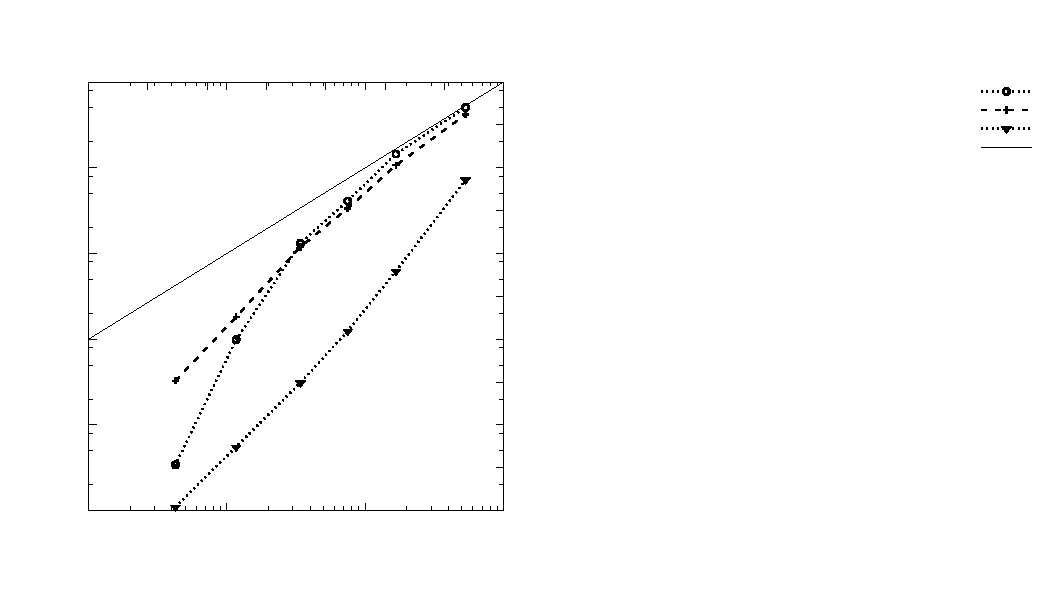
\includegraphics{NodePerformance}}%
    \gplfronttext
  \end{picture}%
\endgroup

	\end{center}
	\caption{
		Solver runtime vs. DoFs, for polynomial degree $k=2/1$,
		for problem/Equation (\ref{eq:NavierStokesCavityBenchmark}).
	}
	\label{fig:DrivenCavity}
\end{figure}